\documentclass[aspectratio=169,9pt]{beamer}

\usepackage[utf8]{inputenc}
\usepackage{amssymb,latexsym,amsmath}
\usepackage{graphicx}
\graphicspath{ {./figures/} }
\usepackage{caption}
\usepackage{subcaption}
\captionsetup{font=tiny,labelfont=tiny}
\usepackage[style=apa,
			sorting=nyt,
			date=year,
			bibencoding=utf8,
			isbn=false,
			eprint=false,
			dashed=false,
			uniquelist=false,
			maxbibnames=10,
			minbibnames=1,
			maxcitenames=2,
			uniquename=init,
			giveninits=true,
			useprefix=false,
			minsortnames=1,
			maxsortnames=2]{biblatex}
\renewcommand*{\bibfont}{\footnotesize}
\renewcommand*{\citesetup}{\tiny}
\renewcommand{\cite}{\parencite}
\bibliography{References}
\usepackage[strict]{changepage}

% Beamer theme
\usetheme[titleformat=smallcaps,
			sectionpage=progressbar,
			subsectionpage=progressbar,
			progressbar=frametitle,
			numbering=fraction]{metropolis}
% FiraFonts if using pdflatex
% \usepackage{FiraSans}
% \usepackage{FiraMono}

\setbeamertemplate{footline}{}
\setbeamertemplate{navigation symbols}{%
    \ifnum\insertframenumber>0
        \footnotesize\insertframenumber/\inserttotalframenumber%
    \fi%
}
% Information to be included in the title page:
\title[Thesis Defence]{A theoretical study of the implications of resource competition for adaptive therapy of castration-resistant prostate cancer}
\subtitle{Thesis Defence}
\author[Harshavardhan BV]{Harshavardhan BV\\
Supervisor: Prof. Sutirth Dey}
\date{July 2021}
\institute{IISER Pune}

\begin{document}

\frame{\titlepage}

\section{Introduction}

\begin{frame}{Conventional and adaptive Therapy}
  \begin{columns}
    \begin{column}{0.45\textwidth}
      \begin{itemize}
        \item Conventional therapy @ MTD $\rightarrow$\\
        $\downarrow$ tumour burden \cite{Frei}
        \item Heterogenous sensitivity $\rightarrow$\\
        sens. $\times$ $\rightarrow$ resst. \cite{Scott}
        \item AT = $\downarrow$ , $\sim$ dose $\rightarrow$ sens. $\checkmark$ \cite{Gatenby}
        \item Drug holiday - sens. $\rightarrow\ \downarrow$ resst.
        \item AT outcome $\leftarrow$ competition
      \end{itemize}
    \end{column}
    \begin{column}{0.55\textwidth}
      \begin{figure}[h]
        \centering
        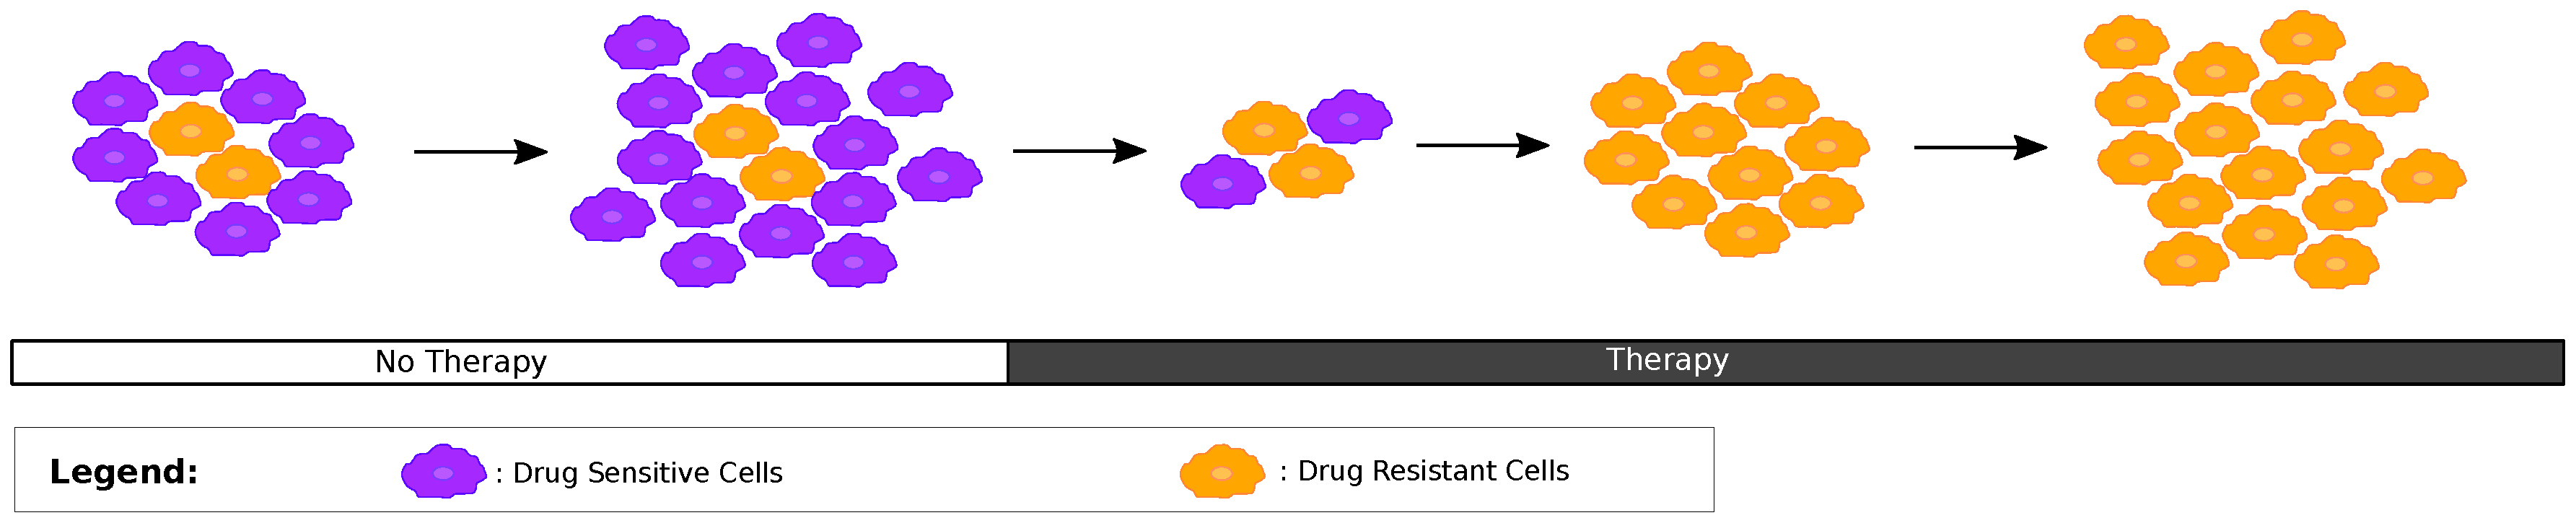
\includegraphics[width=\textwidth]{compe_release}
        \caption{Competitive release under SOC}
      \end{figure}
      \begin{figure}[h]
        \centering
        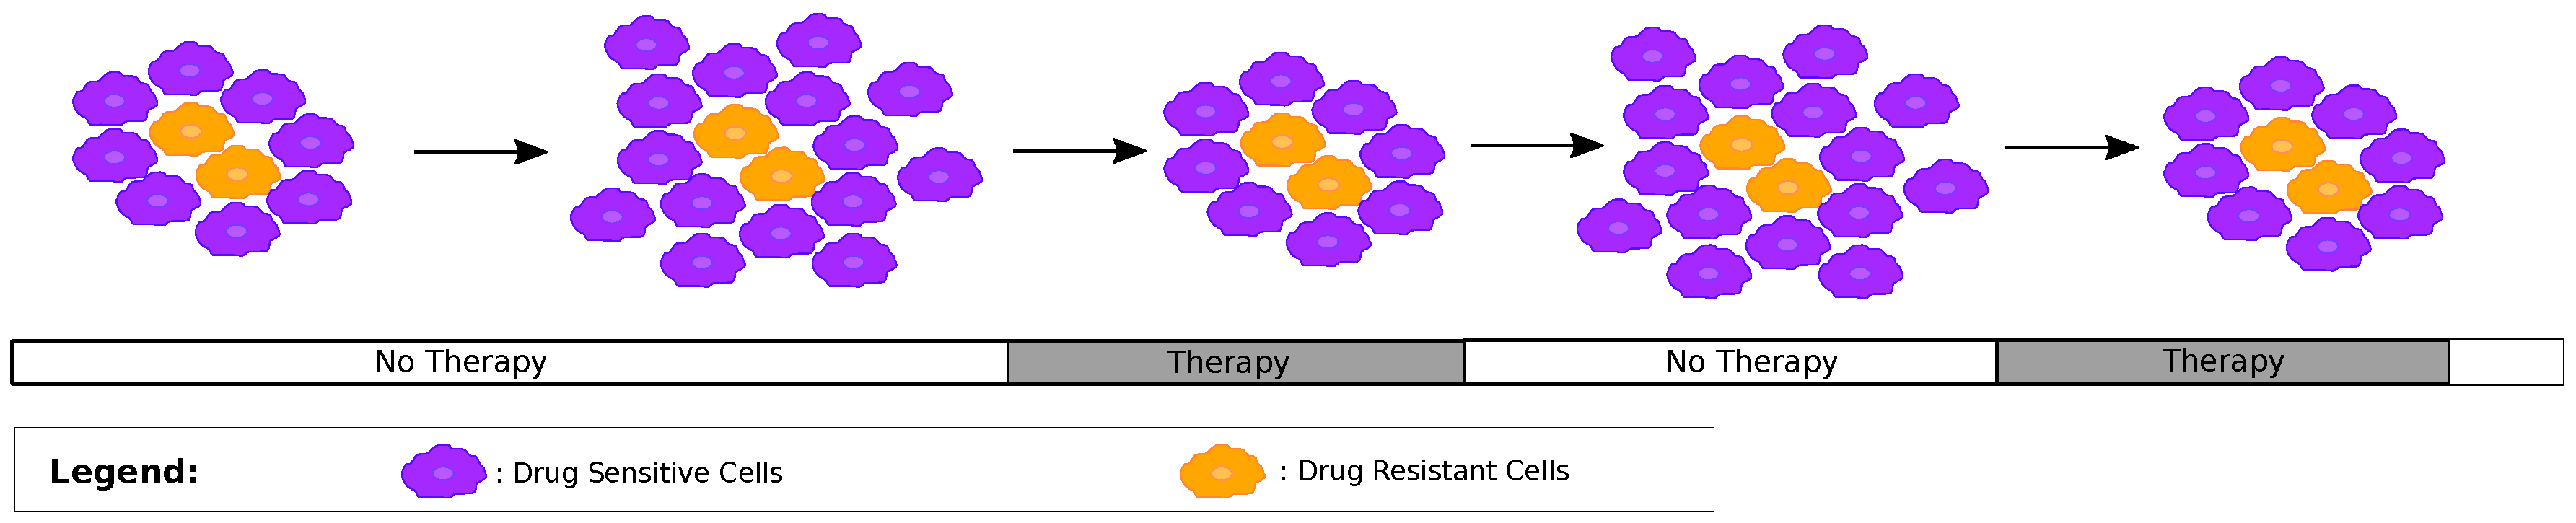
\includegraphics[width=\textwidth]{at}
        \caption{Control under AT}
      \end{figure}
    \end{column}
  \end{columns}
\end{frame}

\begin{frame}{System of study}
  \begin{itemize}
    \item Castration-Resistant Prostate Cancer (CRPC)
    \item AR pathway: prostate cells $\rightarrow$ cancer \cite{Heinlein}
    \item Therapy: ADT + Abiraterone
  \end{itemize}
  \begin{table}
    \centering
    \begin{tabular}{|l|c|c|c|c|}
    \hline
    Cell type & Test. dependent & Test. Producing & Ab. sensitive & Mechanism \\
    \hline
    $T^+$ & Yes & No & Yes & N/A \\
    $T^p$ & Yes & Yes & Yes & Cholesterol $\xrightarrow{CYP17\alpha}$ Test.\\
    $T^-$ & No & No & No & AR $\mu^n$\\
    \hline
    \end{tabular}
  \end{table}
\end{frame}

\begin{frame}{System of equations}
  \begin{columns}
    \begin{column}{0.45\textwidth}
      \begin{itemize}
        \item Logistic framework w/ dynamic carrying capacity $\approx$ env. condn.
        \item Environment = resource = $\{O_2,test\}$
        \item No $\mu^n$, no spatial structure, well mixed
        \item Defined $\mathbb{R}_{\geq 0}$, $y_i < 1 =$ extinction
      \end{itemize}
      \begin{figure}[h]
        \centering
        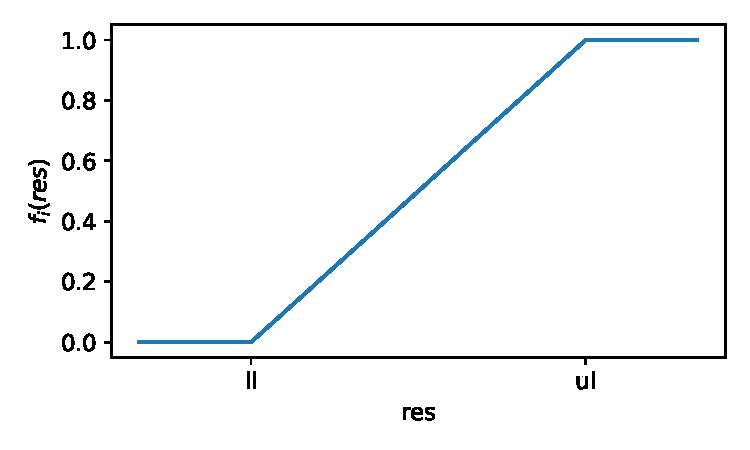
\includegraphics[width=\textwidth]{f_res}
        \caption{$f_i(res)$}
      \end{figure}
    \end{column}
    \begin{column}{0.55\textwidth}
      \begin{equation}
        \frac{dy_i}{dt} = r_i y_i (1 - \frac{\sum_j y_j}{1 + K_{i,max} f_i(O_2) f_i(test)} )- \delta_i y_i
        \label{celleq}
      \end{equation}
      \begin{equation}
        \frac{dO_2}{dt} = p_{O_2} - \sum_i \mu_{O_2,i} y_i - \lambda_{O_2} O_2
        \label{o2eq}
      \end{equation}
      \begin{equation}
        \frac{dtest}{dt} = p_{test} y_{T^p} - \sum_i \mu_{test,i} y_i - \lambda_{test} test
        \label{testeq}
      \end{equation}
      \begin{equation}
        f_i(res) = \begin{cases}
          1 &\text{if } ul_{res,i} \leq res\\
          \frac{res-ll_{res,i}}{ul_{res,i}-ll_{res,i}} &\text{if } ll_{res,i} < res < ul_{res,i}\\
          0 &\text{if } res \leq ll_{res,i}\\
        \end{cases}
        \label{freseq}
      \end{equation}
      $i \in \{T^+,T^p,T^-\}$ and $res \in \{O_2,test\}$.
    \end{column}
  \end{columns}
\end{frame}


\section{What happens in the absence of therapy?}

\begin{frame}{All cell-type competition outcomes}
  \begin{figure}[h]
    \begin{adjustwidth}{-5cm}{-5cm}
      \centering
      \begin{subfigure}[b]{0.53\textwidth}
        \centering
        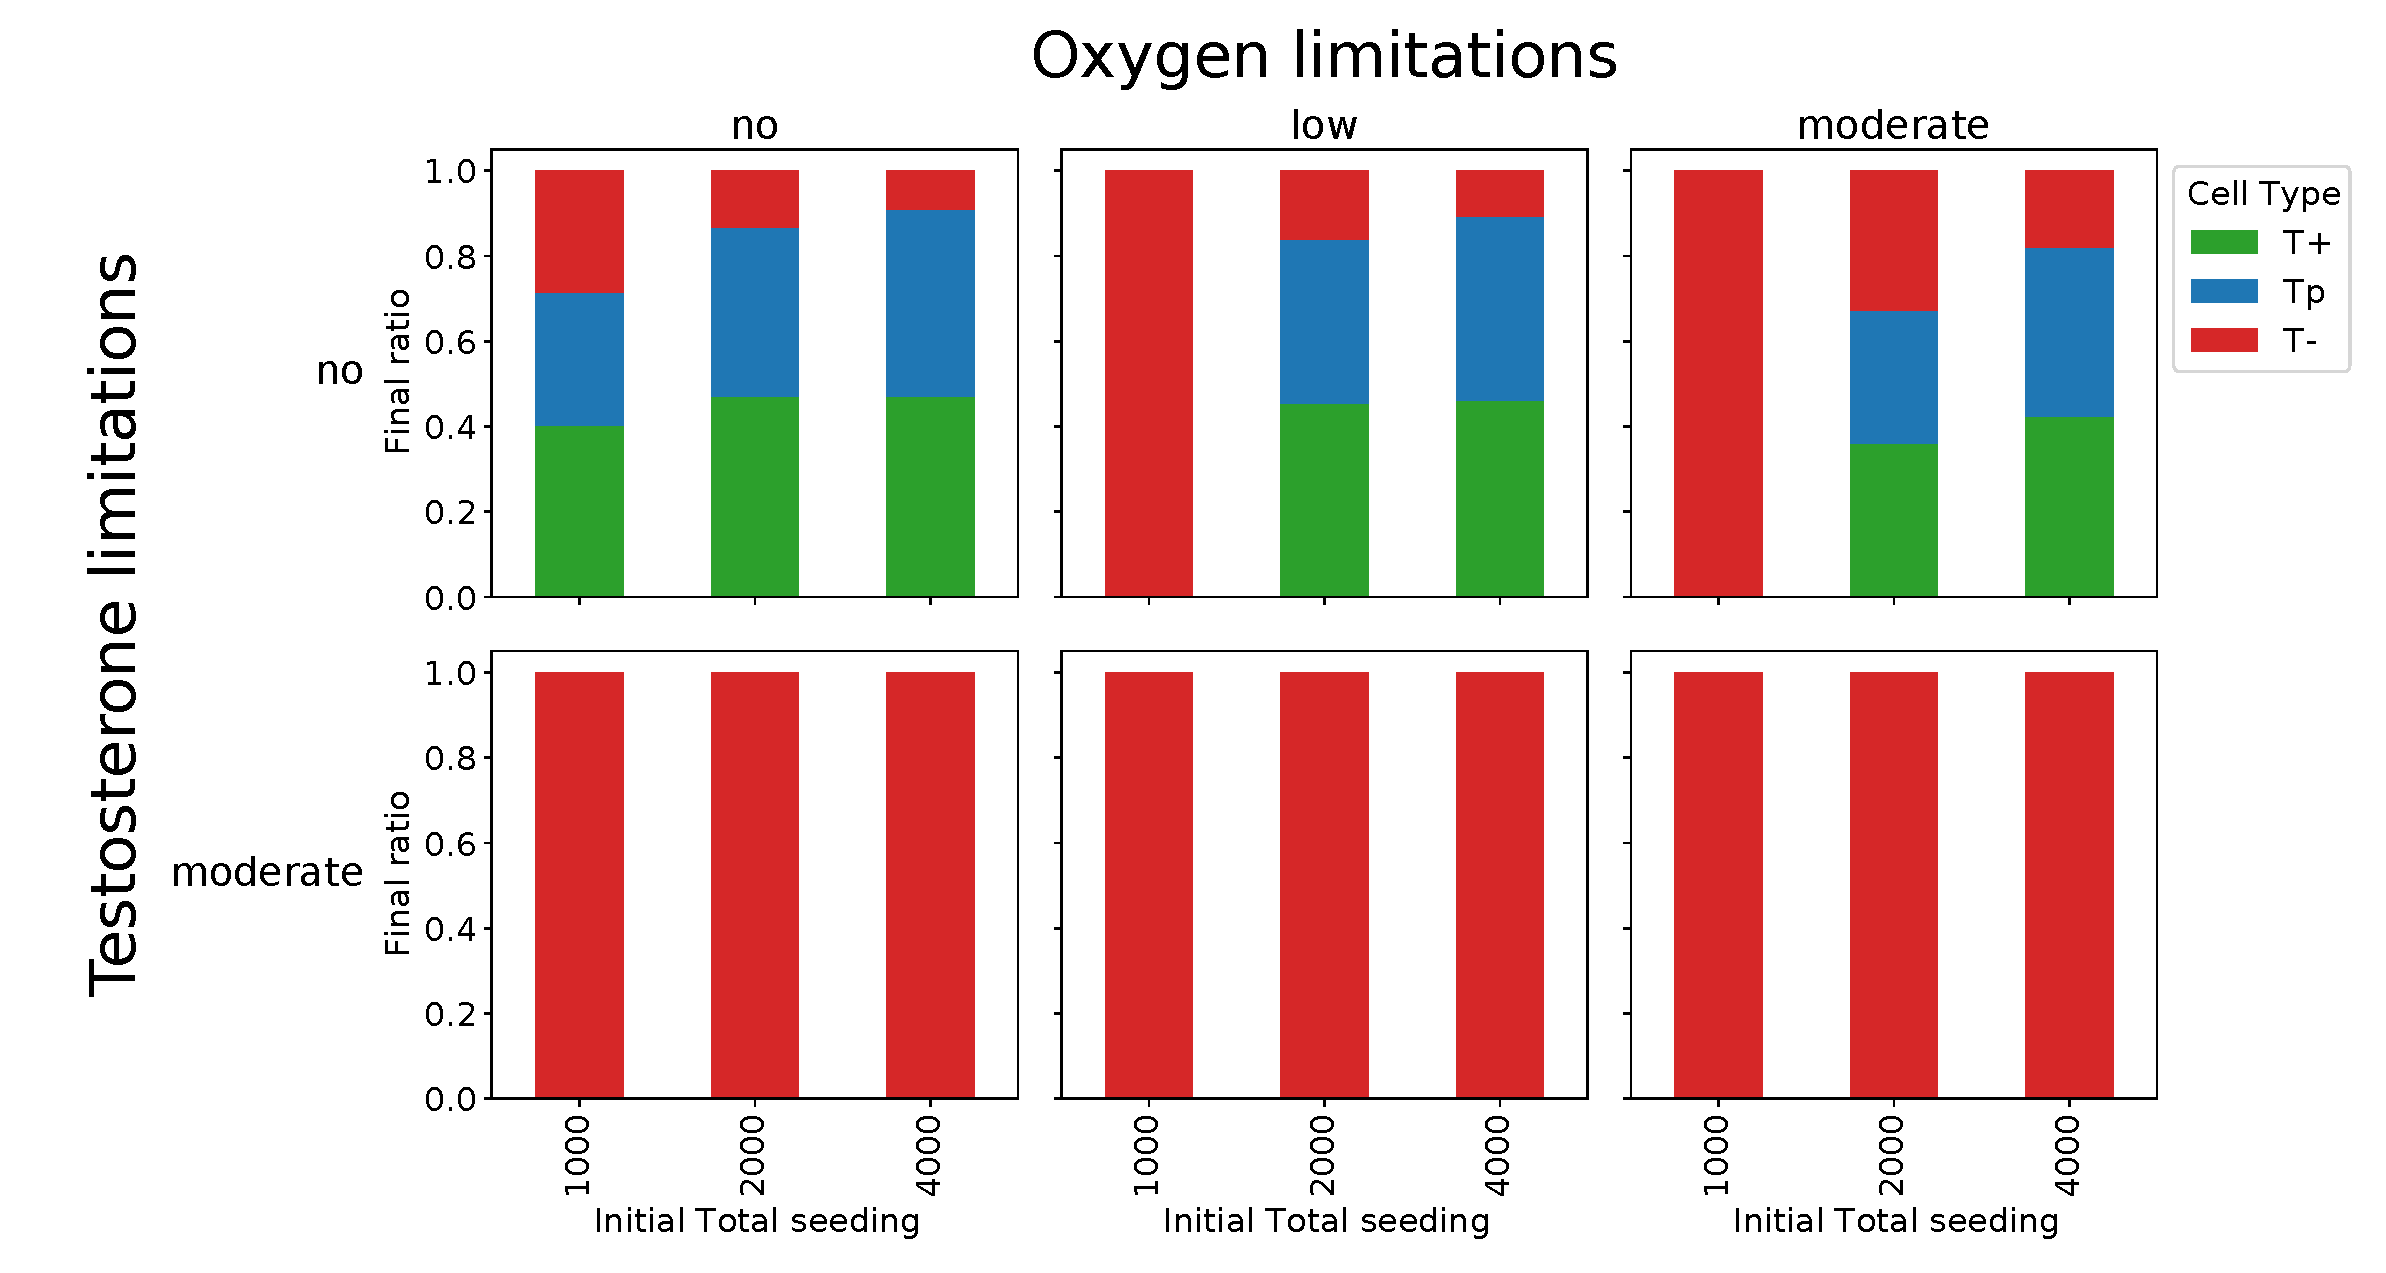
\includegraphics[width=\textwidth]{All3_efficiency_1:1:1}
        \caption{Equal seeding - 1:1:1 }
      \end{subfigure}
      \begin{subfigure}[b]{0.53\textwidth}
        \centering
        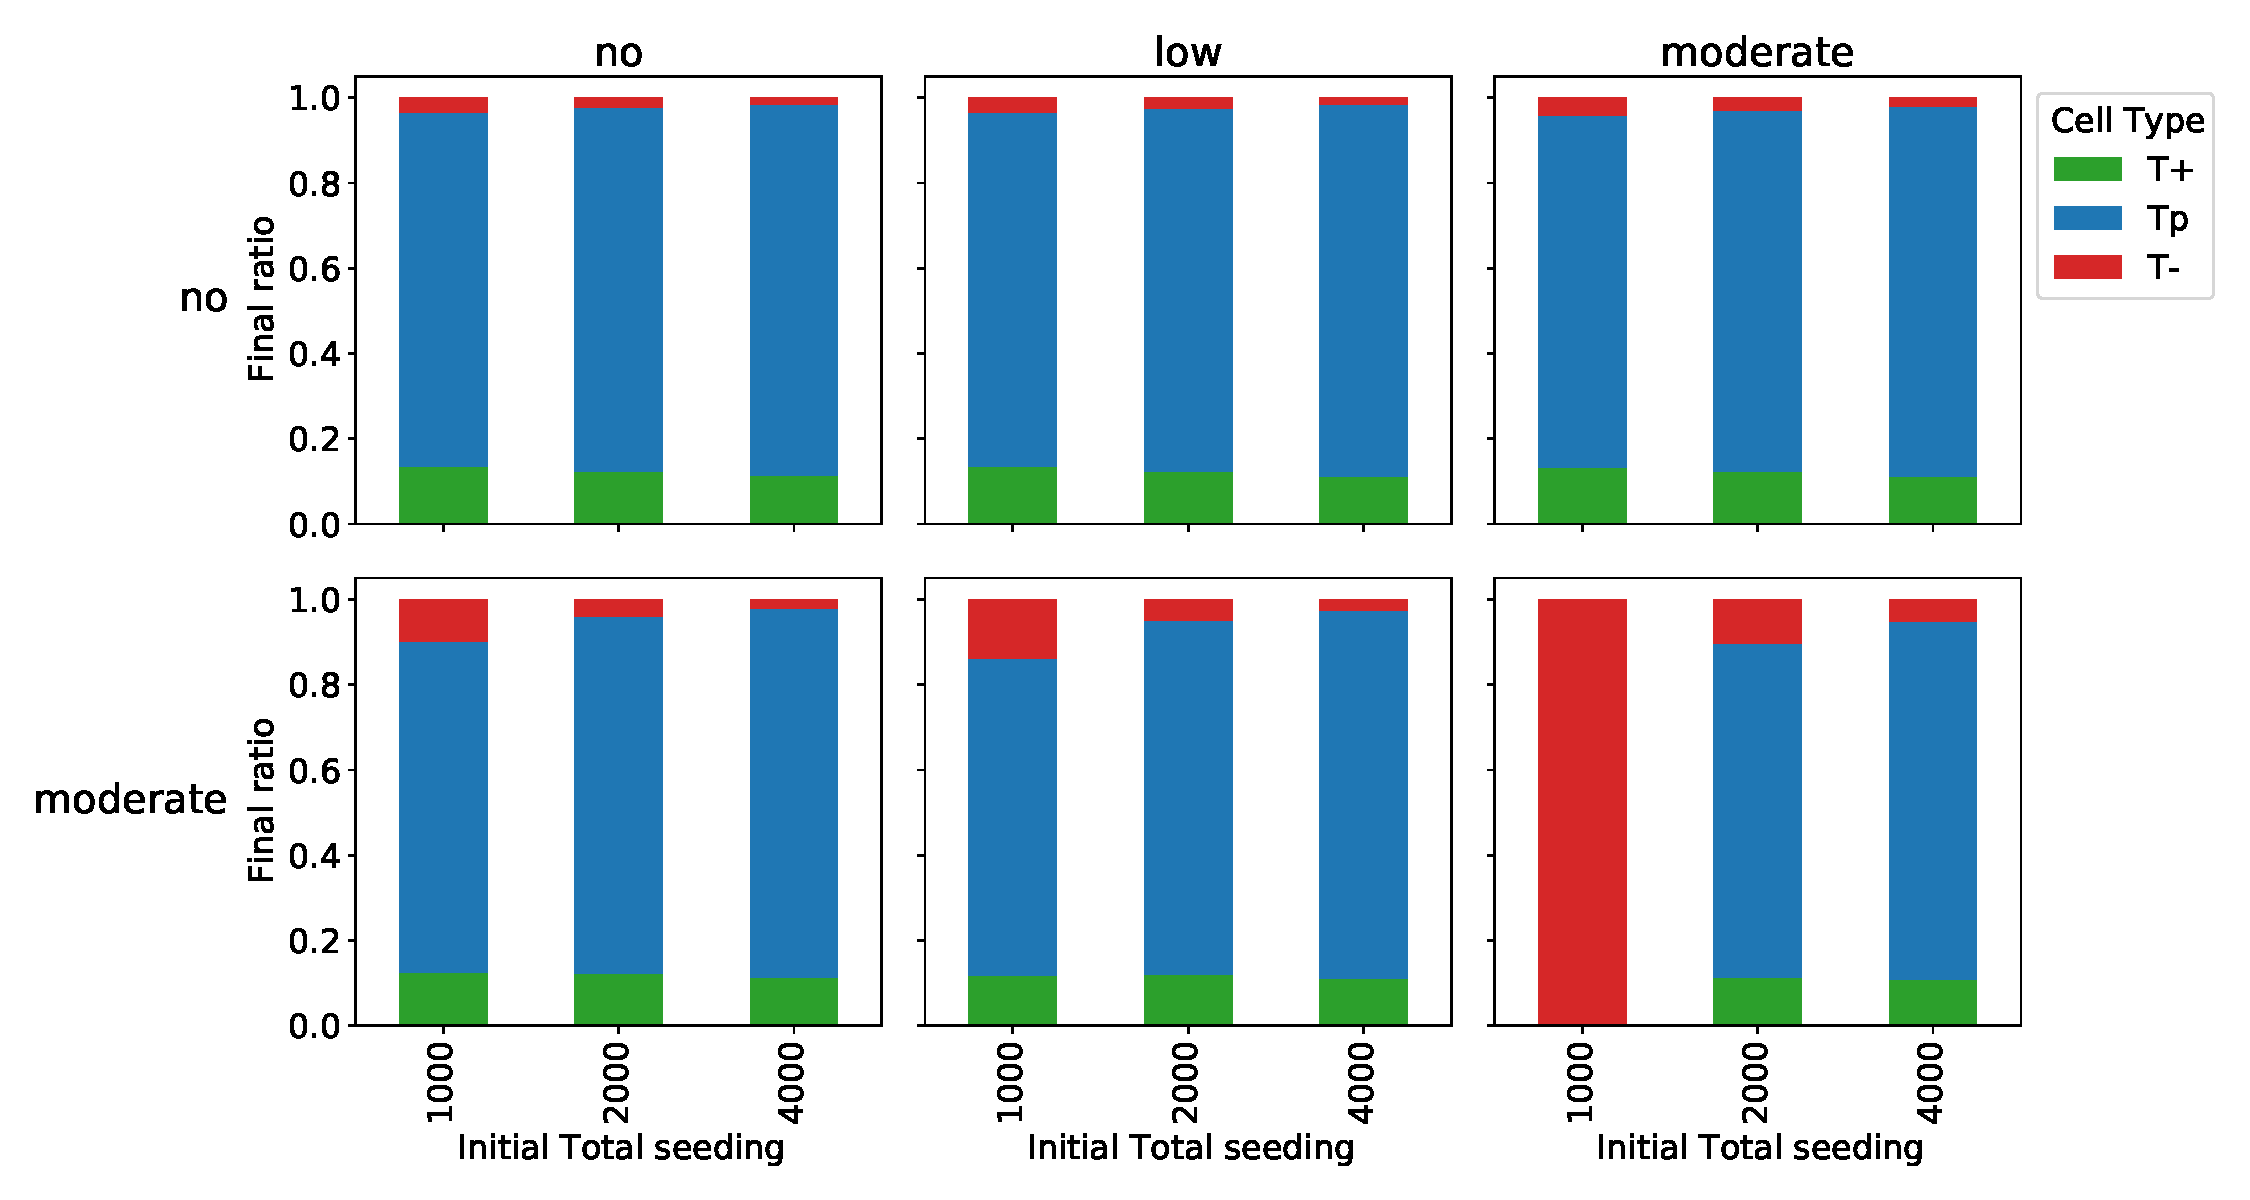
\includegraphics[width=\textwidth]{All3_efficiency_8:1:1}
        \caption{High $T^p$ seeding - 8:1:1}
      \end{subfigure}
    \end{adjustwidth}
    \caption{Final ratio of all cell types. (Stacked bar plot)}
  \end{figure}
  \begin{columns}
    \begin{column}{0.5\textwidth}
      \begin{itemize}
        \item<1-> All the cells have the same limitations
        \item<2-> Higher $T^p$ seeding ratios $\Rightarrow$ increased testosterone production
        \item<3-> Coexistence is important: tumour with $T^p$ and $T^+$ would only respond to therapy
      \end{itemize}
    \end{column}
    \begin{column}{0.5\textwidth}
      \begin{itemize}
        \item<4-> Testosterone: drastic effect on coexistence as only $T^p -T^+$ affected
        \item<5-> Oxygen: minor effect, pushes to extinction if combined limitation on the edge
      \end{itemize}
    \end{column}
  \end{columns}
\end{frame}

\section{What happens when we add therapy?}

\begin{frame}{How is it implemented?}
  \begin{columns}
    \begin{column}{0.43\textwidth}
      \begin{itemize}
        \item<1-> Therapy: modelled as boolean
        \begin{equation}
          \begin{aligned}
            & 1 = \text{MTD}\\
            & 0 = \text{no dose}
          \end{aligned}
        \end{equation}
        \item<2-> Abiraterone:
        blocks $CYP17\alpha$ \\ $T^p$, $T^+$ affected
        \begin{equation}
          p_{test}(abi) = \begin{cases}
          p_{test,max} &\text{if } abi = 0 \\
          p_{test,min} &\text{if } abi = 1 \\
          \end{cases}
          \label{p_test_dose_eq}
        \end{equation}

        \item<3-> Docetaxel: disrupts microtubule \\ All 3 affected
        \begin{equation}
          r_i(dtx) = \begin{cases}
          r_{i,max} &\text{if } dtx = 0 \\
          r_{i,min} &\text{if } dtx = 1 \\
          \end{cases}
          \label{r_dose_eq}
        \end{equation}

      \end{itemize}
    \end{column}
    \begin{column}{0.6\textwidth}
      \begin{itemize}
        \item<4-> SOC\footnotemark[1]: dose given at MTD\footnotemark[1] from the beginning
        \begin{equation}
          dose(y,t) = 1 \quad \forall\ t, y
          \label{dose_soc_eq}
        \end{equation}
        \item<5-> AT\footnotemark[1]: binary mode considered
        \begin{itemize}
          \item Dose at MTD\footnotemark[1] when on
          \item Therapy turned on when population above On threshold
          \item Therapy turned off when population below Off threshold
        \end{itemize}
        \begin{equation}
          dose(y,t) = \begin{cases}
          0 &\text{if } dose(y,t-\Delta t) = 0 \text{ and } y < \text{On} \\
          1 &\text{if } dose(y,t-\Delta t) = 0 \text{ and } y \geq \text{On} \\
          1 &\text{if } dose(y,t-\Delta t) = 1 \text{ and } y > \text{Off} \\
          0 &\text{if } dose(y,t-\Delta t) = 1 \text{ and } y \leq \text{Off} \\
          \end{cases}
          \label{dose_at_eq}
        \end{equation}
      \end{itemize}
    \end{column}
  \end{columns}
  \footnotetext[1]{MTD: Maximum tolerated dose, SOC: Standard-Of-Care, AT: Adaptive Therapy}
  \footnotetext[2]{abi: abiraterone, dtx: docetaxel}
\end{frame}

\begin{frame}{What happens with Standard-Of-Care?}
  \begin{figure}[h]
    \begin{adjustwidth}{-5cm}{-5cm}
      \centering
      \begin{subfigure}[b]{0.53\textwidth}
        \centering
        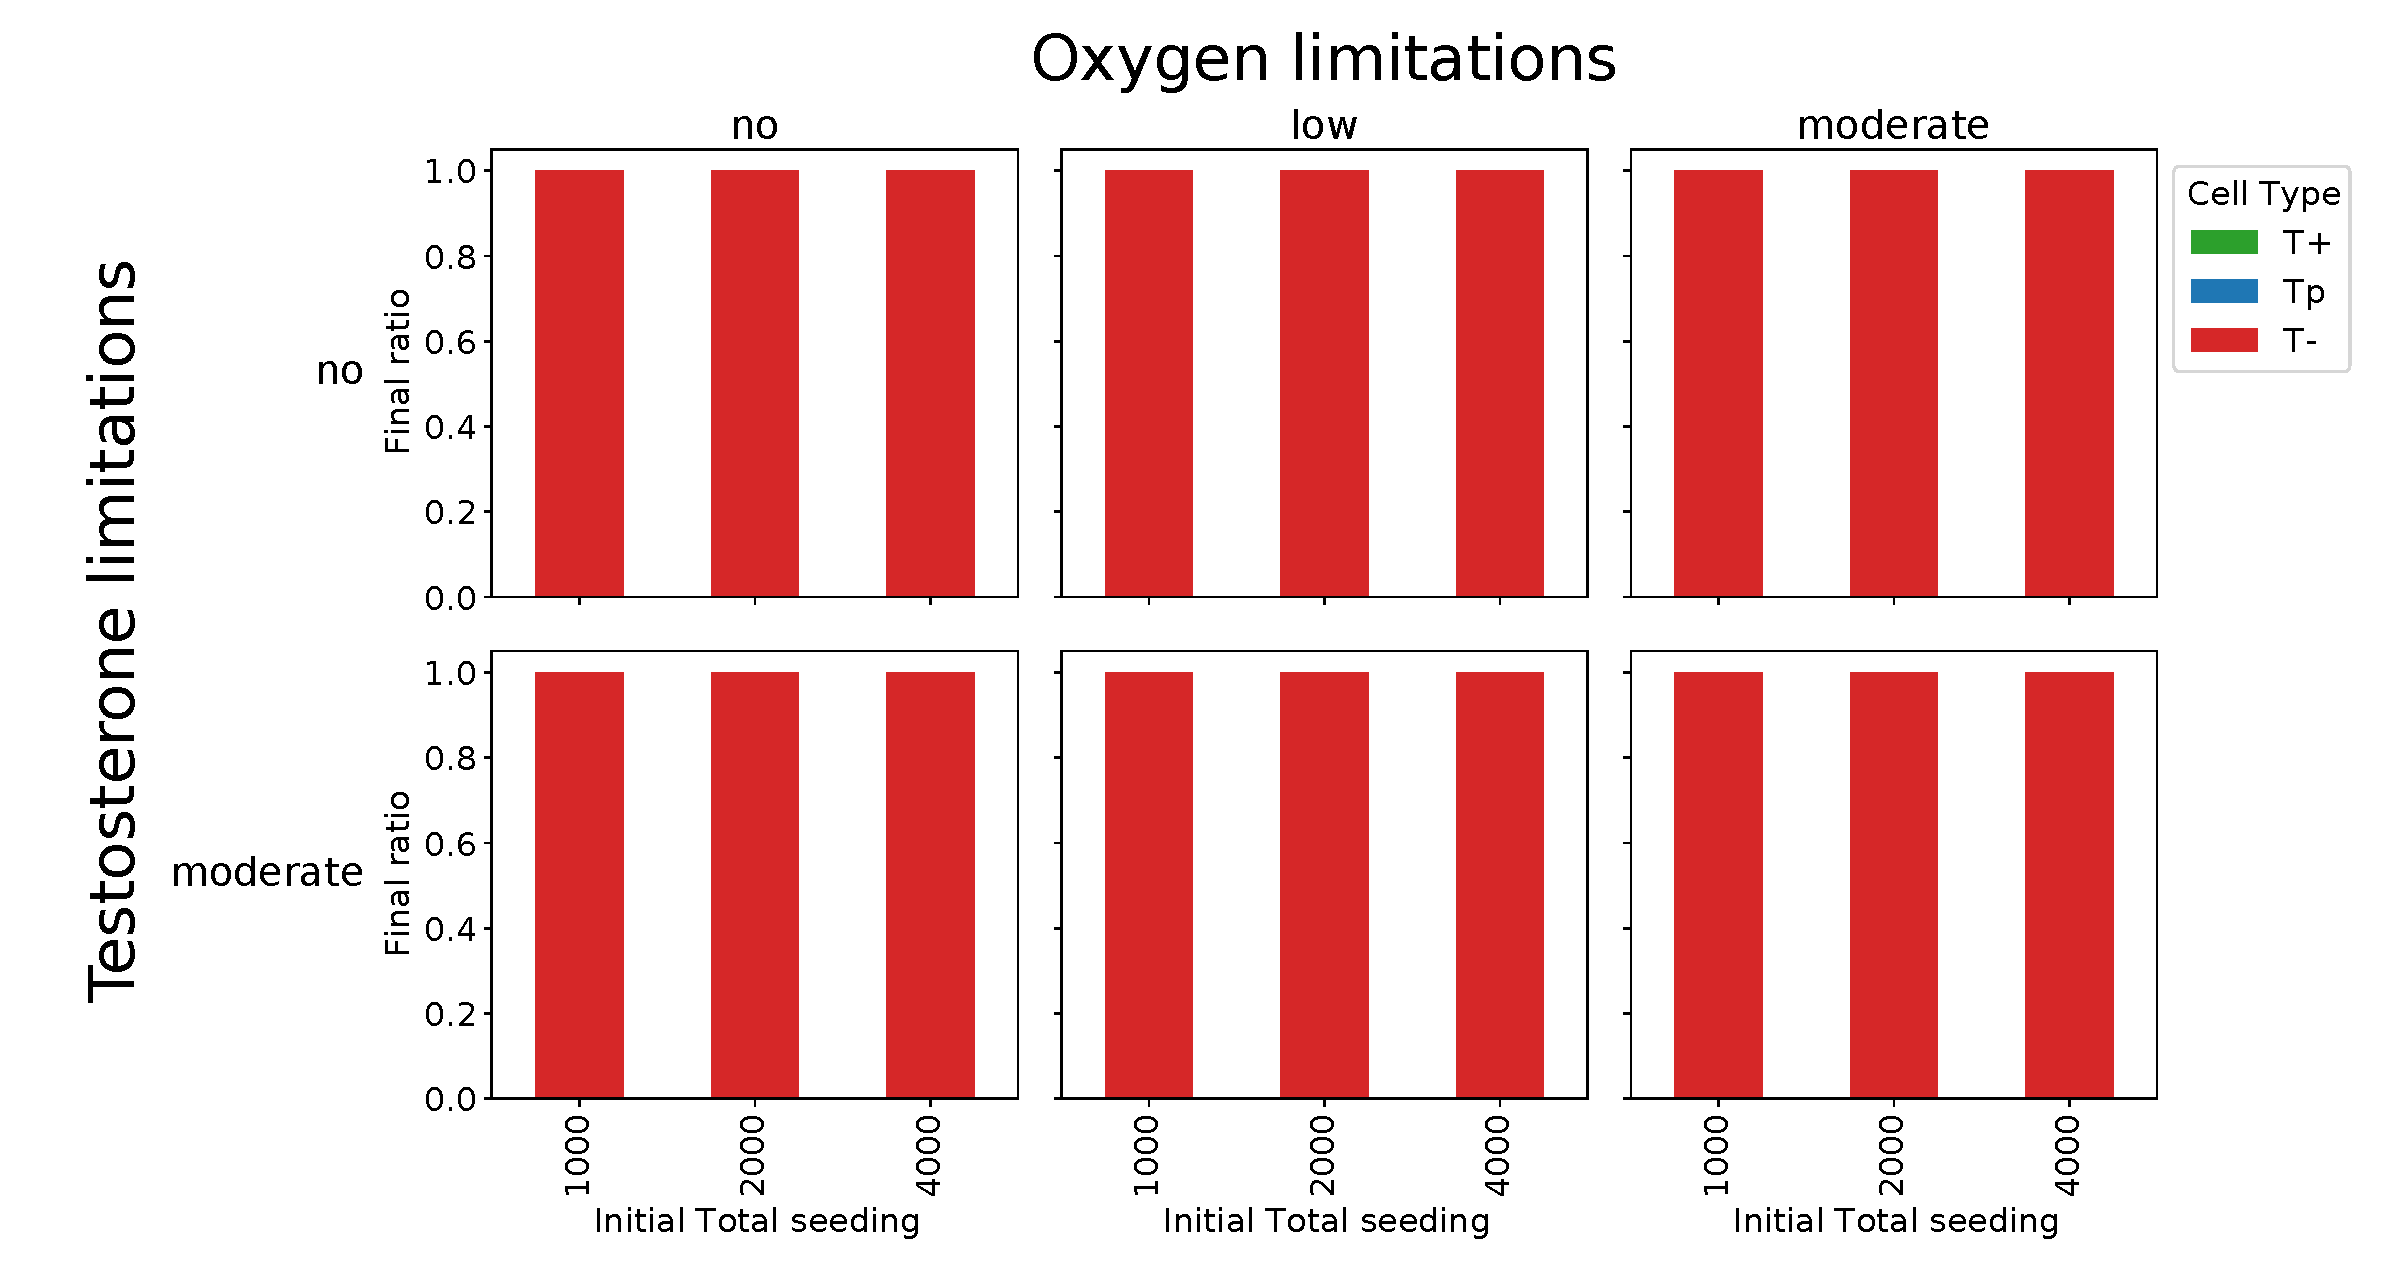
\includegraphics[width=\textwidth]{All3_therapy-SOC_1:1:1}
        \caption{Equal seeding - 1:1:1}
      \end{subfigure}
      \begin{subfigure}[b]{0.53\textwidth}
        \centering
        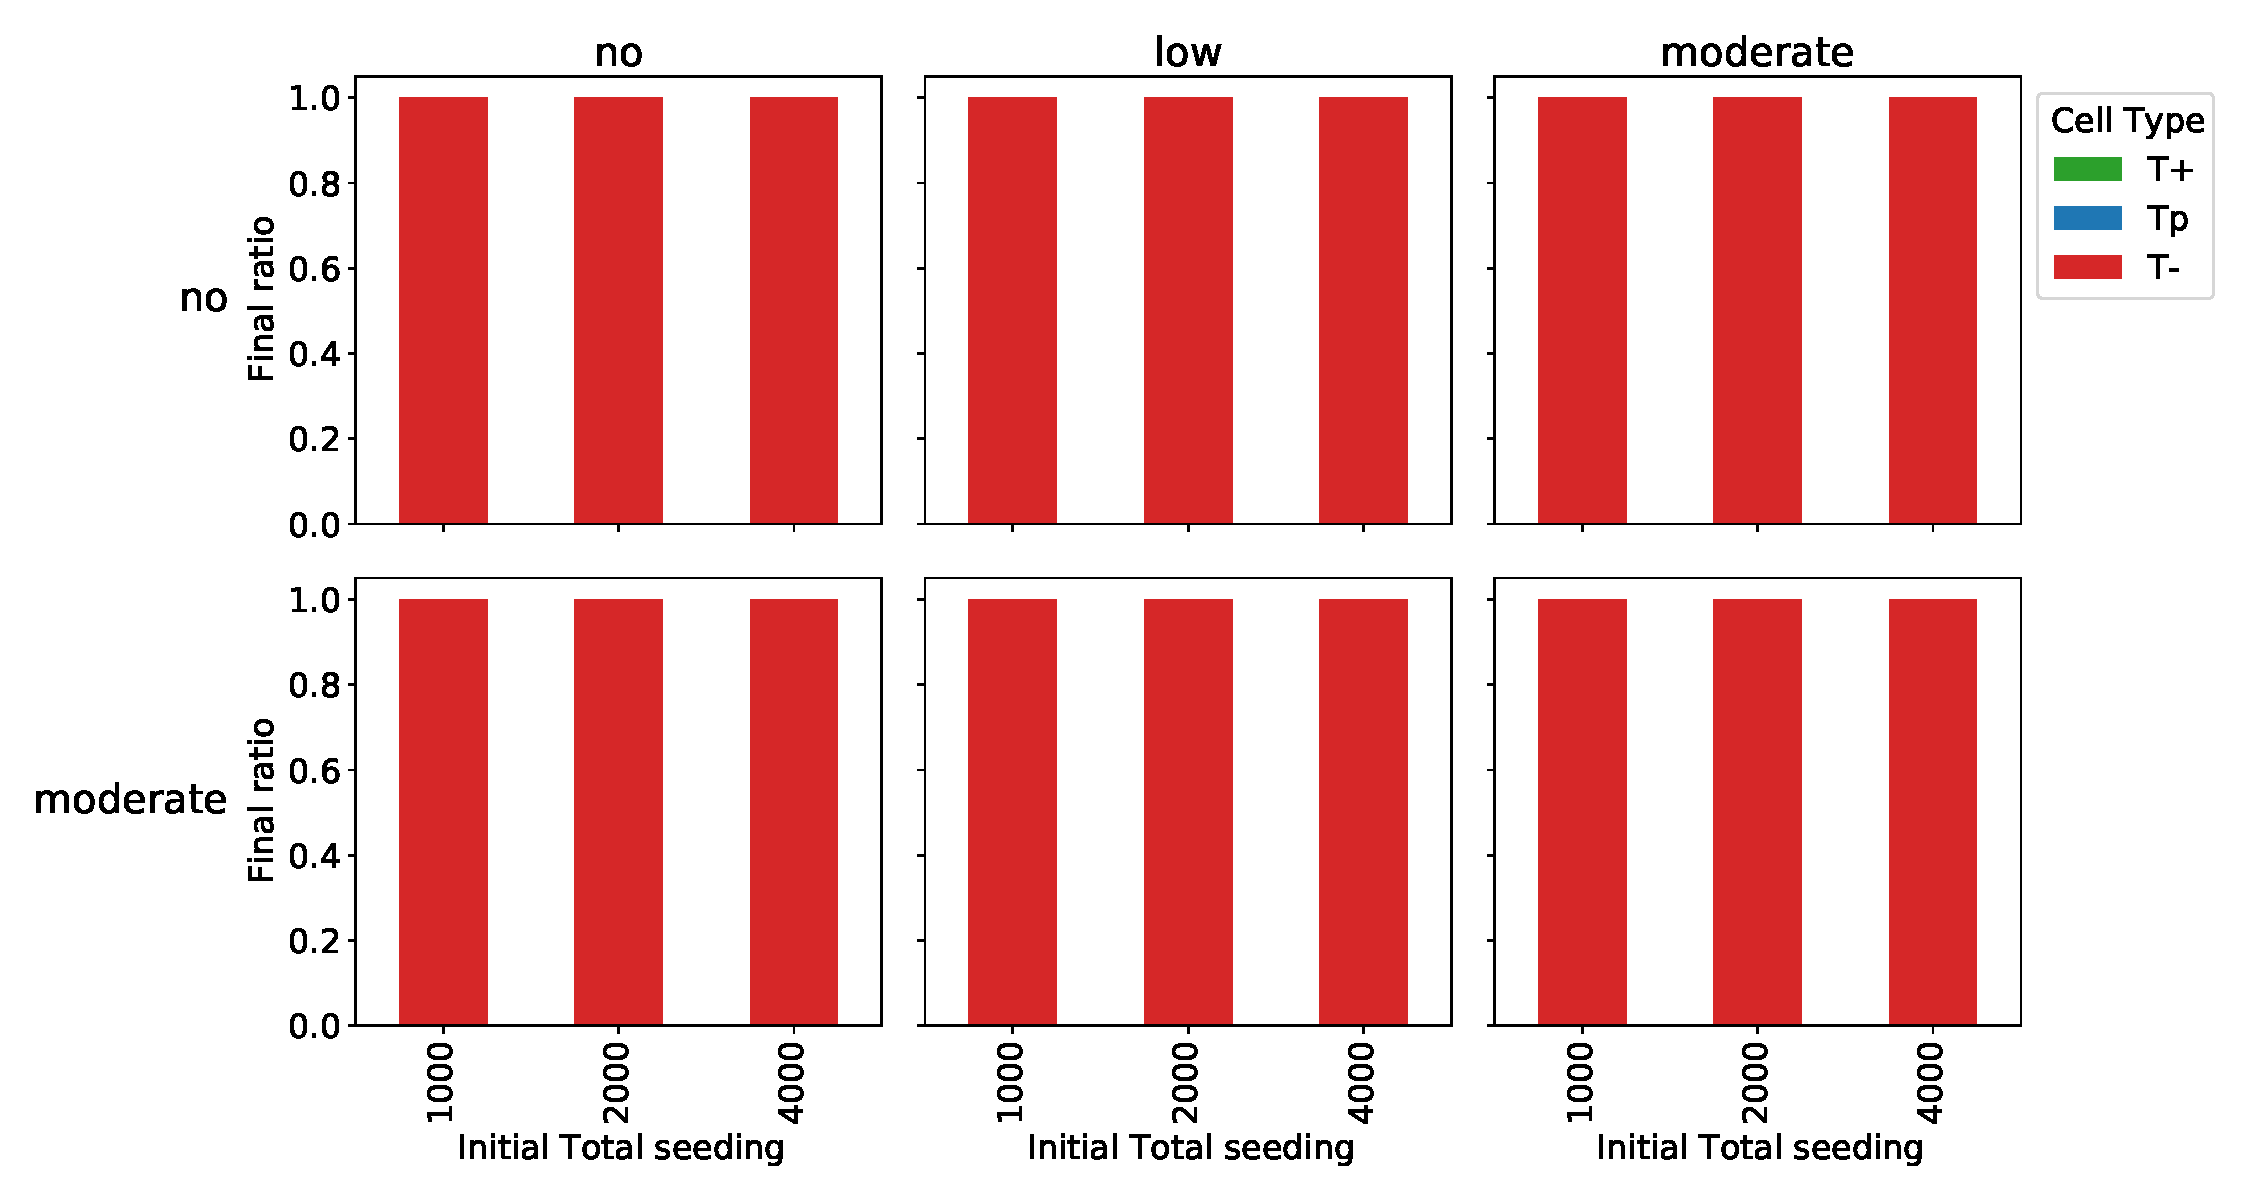
\includegraphics[width=\textwidth]{All3_therapy-SOC_8:1:1}
        \caption{High $T^p$ seeding - 8:1:1}
      \end{subfigure}
    \end{adjustwidth}
    \caption{Final ratio of all cell types under standard-of-care. (Stacked bar plot)}
  \end{figure}
  \begin{columns}
    \begin{column}{0.5\textwidth}
      \begin{itemize}
        \item $T^+, T^p$ go extinct in all cases
      \end{itemize}
    \end{column}
    \begin{column}{0.5\textwidth}
      \begin{itemize}
        \item Testosterone levels insufficient for growth
      \end{itemize}
    \end{column}
  \end{columns}
\end{frame}

\begin{frame}{Thresholds for Adaptive Therapy }
  \begin{figure}[h]
    \centering
    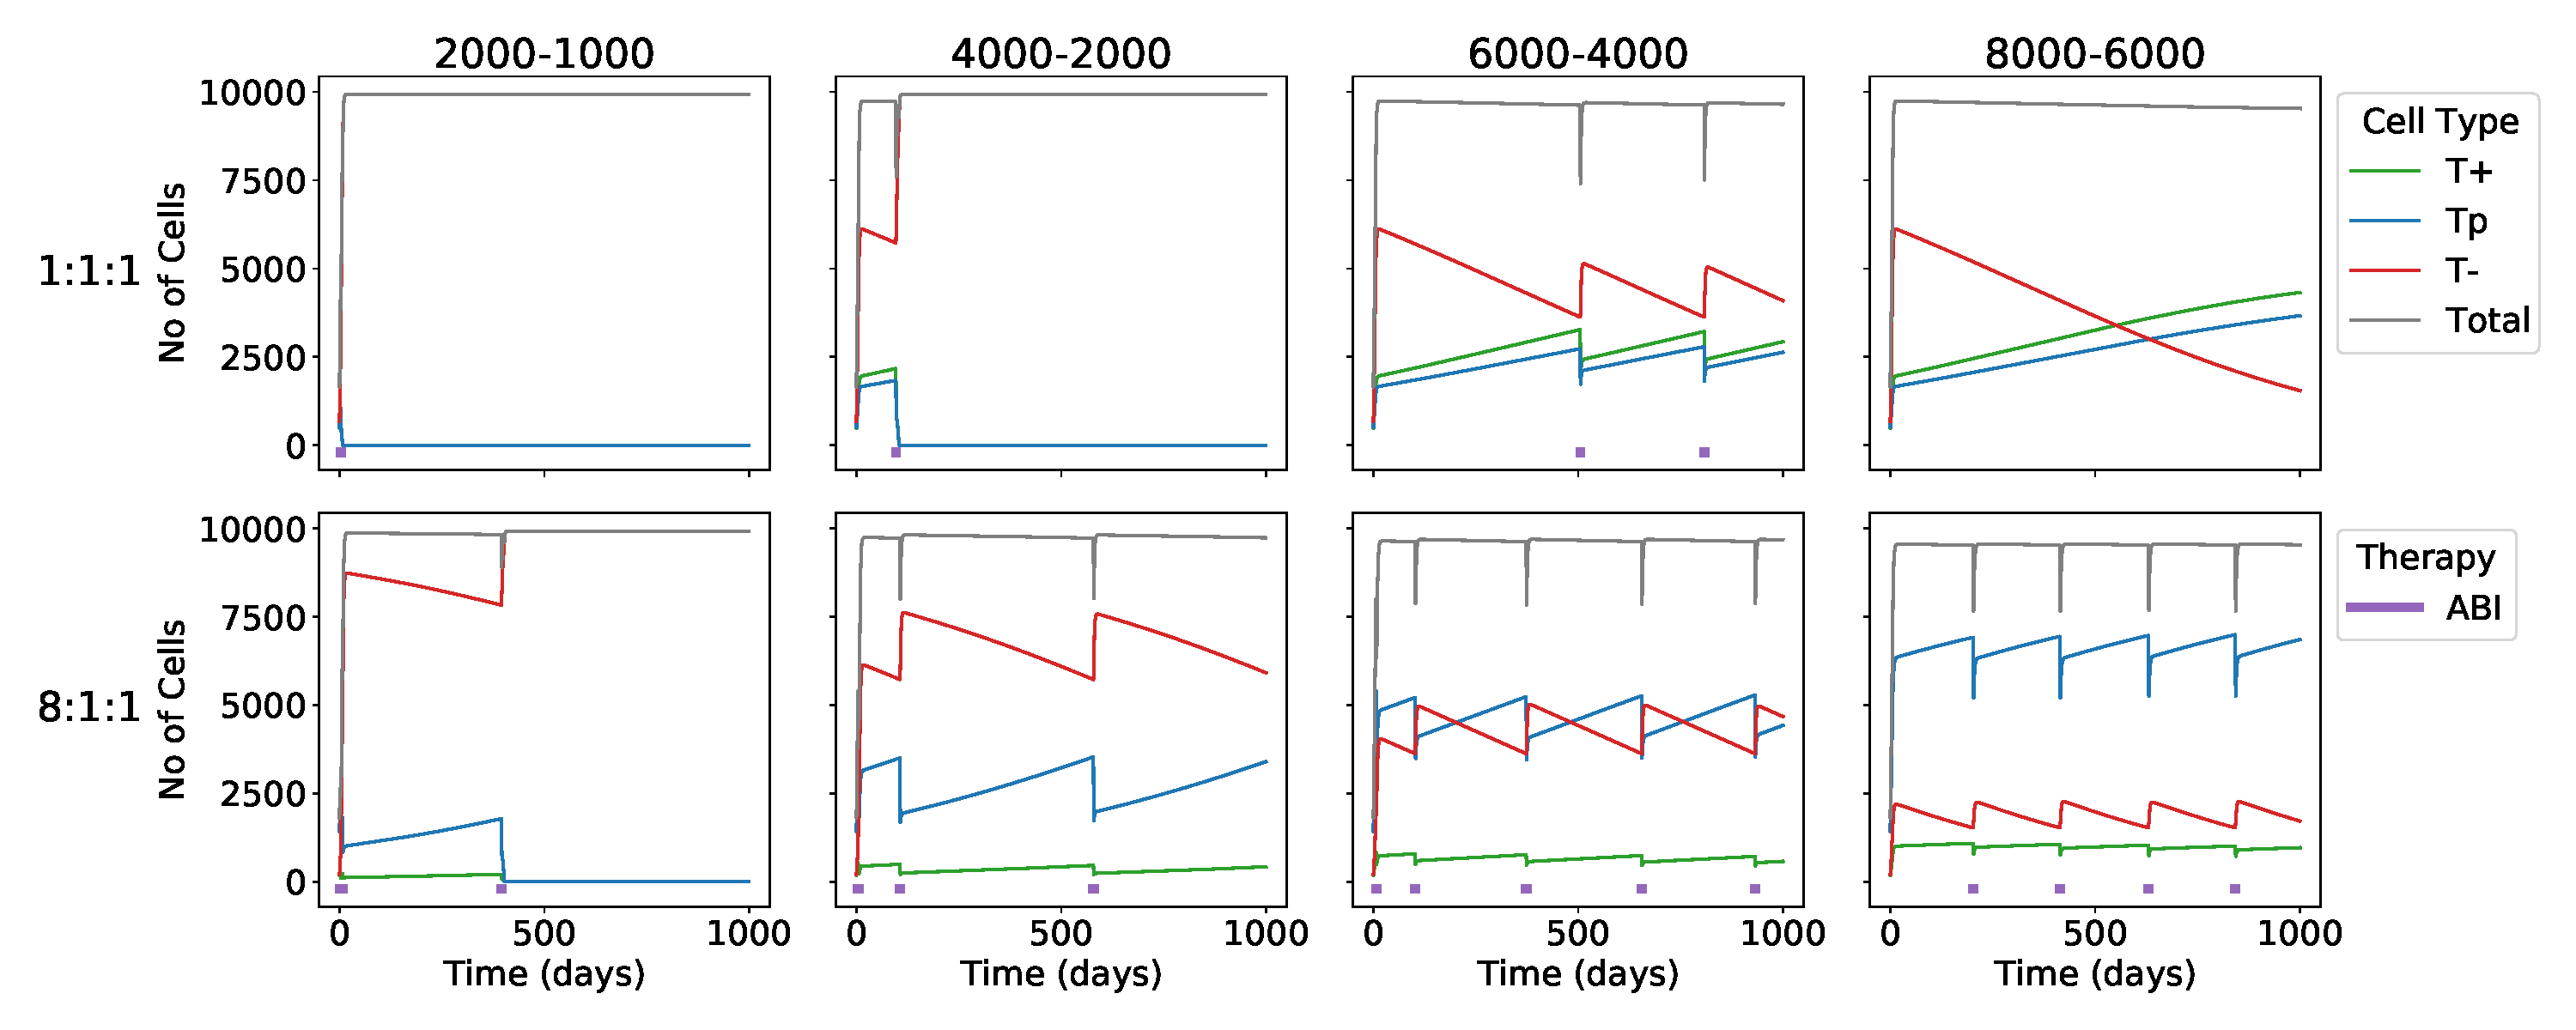
\includegraphics[width=0.7\textwidth]{All3_therapy-standardization}
    \caption{Standardisation of threshold for adaptive therapy}
  \end{figure}
  \begin{columns}
    \begin{column}{0.65\textwidth}
      \begin{itemize}
        \item<1-> Low threshold: $T^-$ inhibits $T^p - T^+$ and causes extinction
        \item<2-> High threshold: $T^+ - T^p$ can compete with $T^-$ \cite{Hansen}
        \item<3-> Too High: No therapy applied as On threshold never crossed
        \item<4-> Chosen- On: 6000, Off: 4000
      \end{itemize}
    \end{column}
    \begin{column}{0.4\textwidth}
      \begin{itemize}
        \item<5-> $T^+ + T^p$ only for threshold
        \item<5-> With total: $T^+ - T^p$ go extinct before therapy turned off
      \end{itemize}
    \end{column}
  \end{columns}
\end{frame}

\begin{frame}{Is Adaptive Therapy better?}
  \begin{figure}[h]
    \begin{adjustwidth}{-5cm}{-5cm}
      \centering
      \begin{subfigure}[b]{0.53\textwidth}
        \centering
        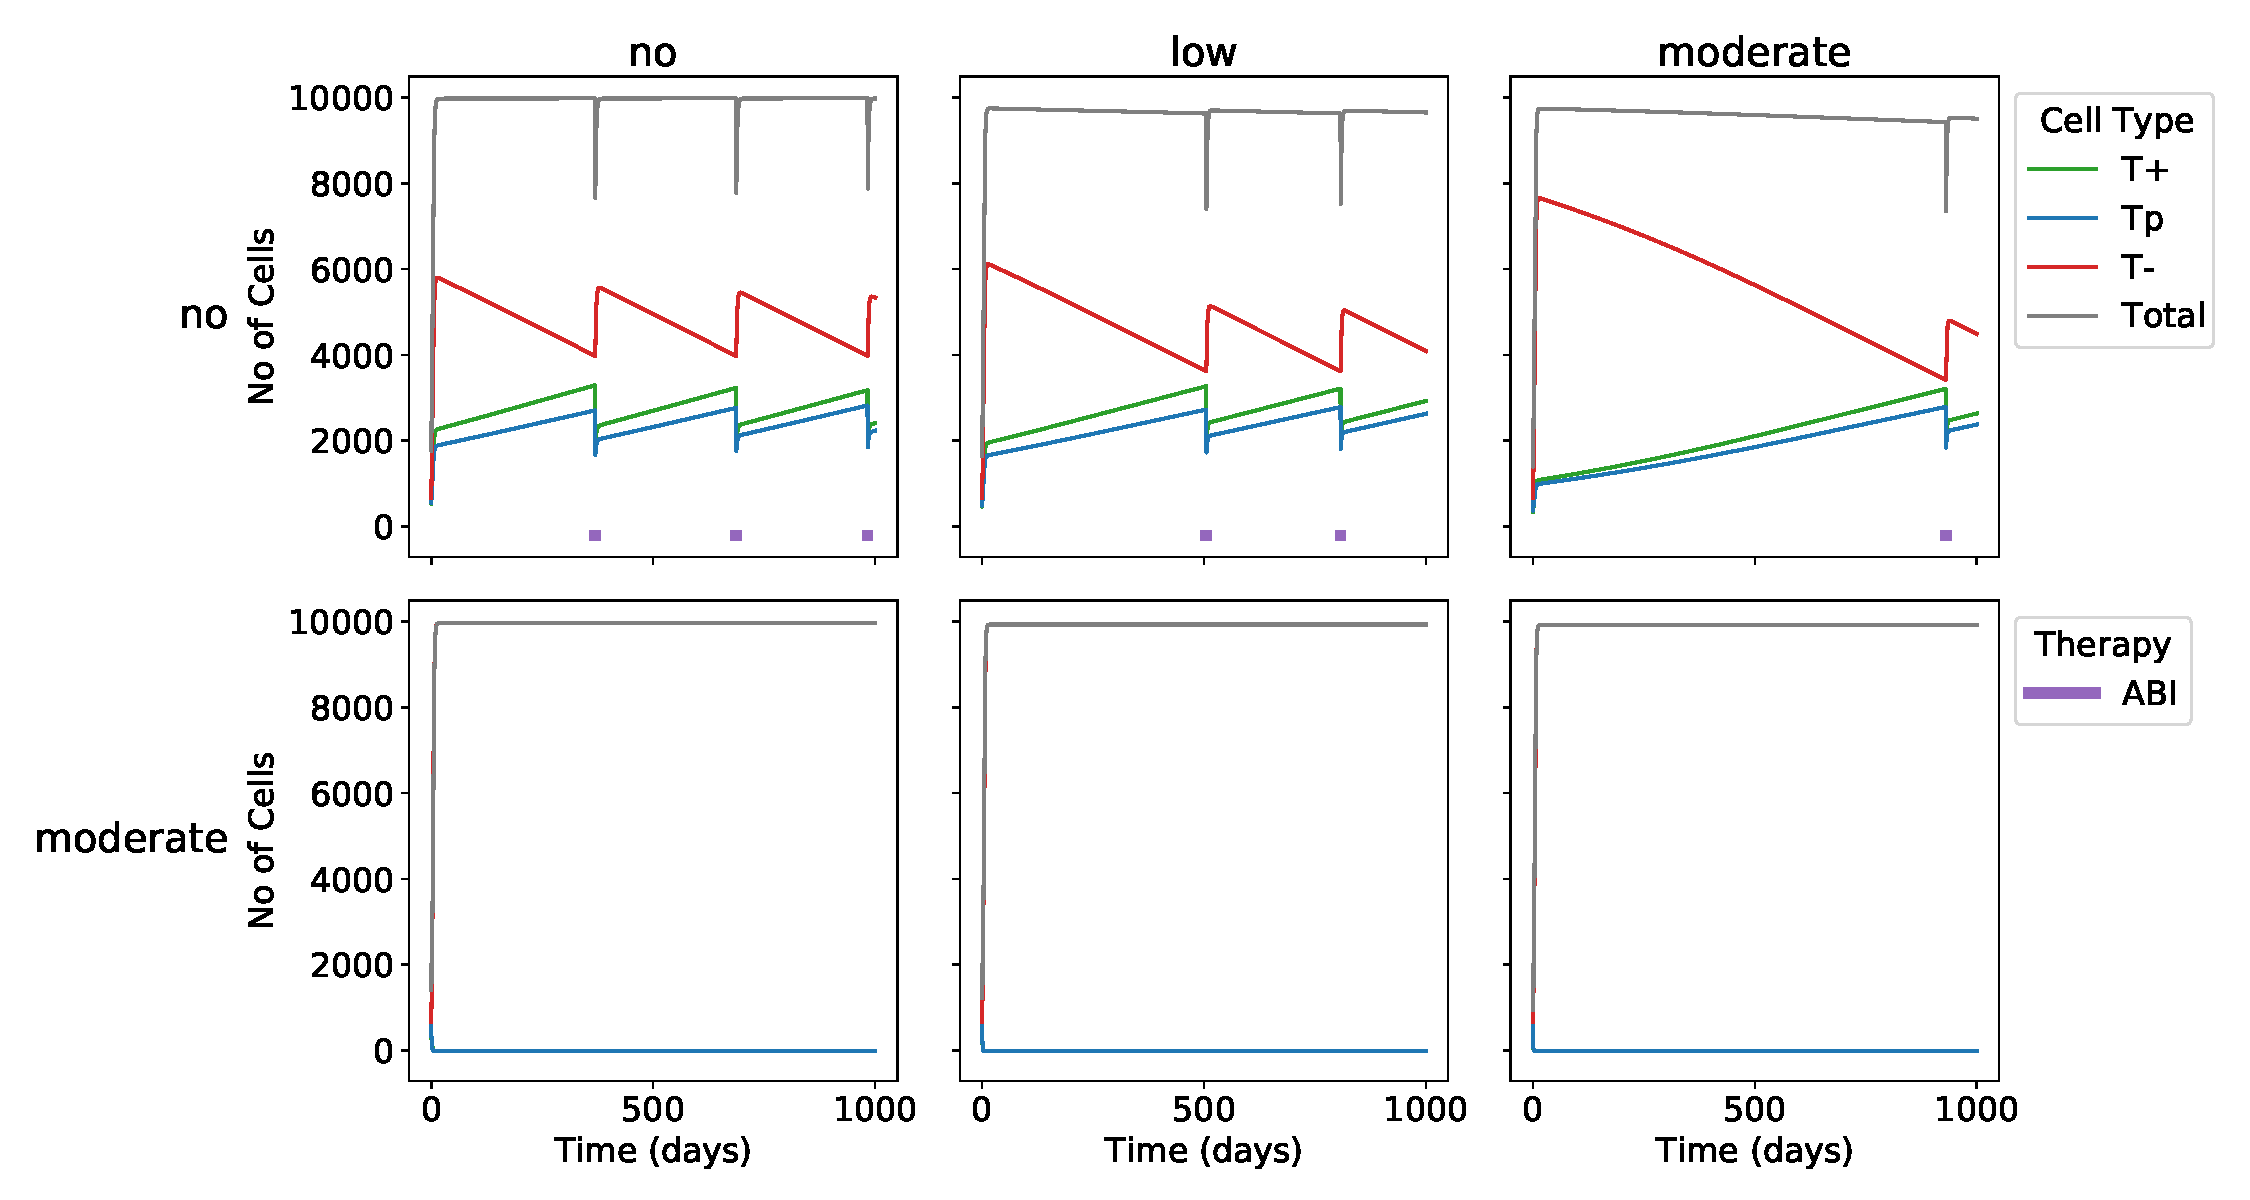
\includegraphics[width=\textwidth]{All3_therapy_1:1:1-2000}
        \caption{Equal seeding - 1:1:1}
      \end{subfigure}
      \begin{subfigure}[b]{0.53\textwidth}
        \centering
        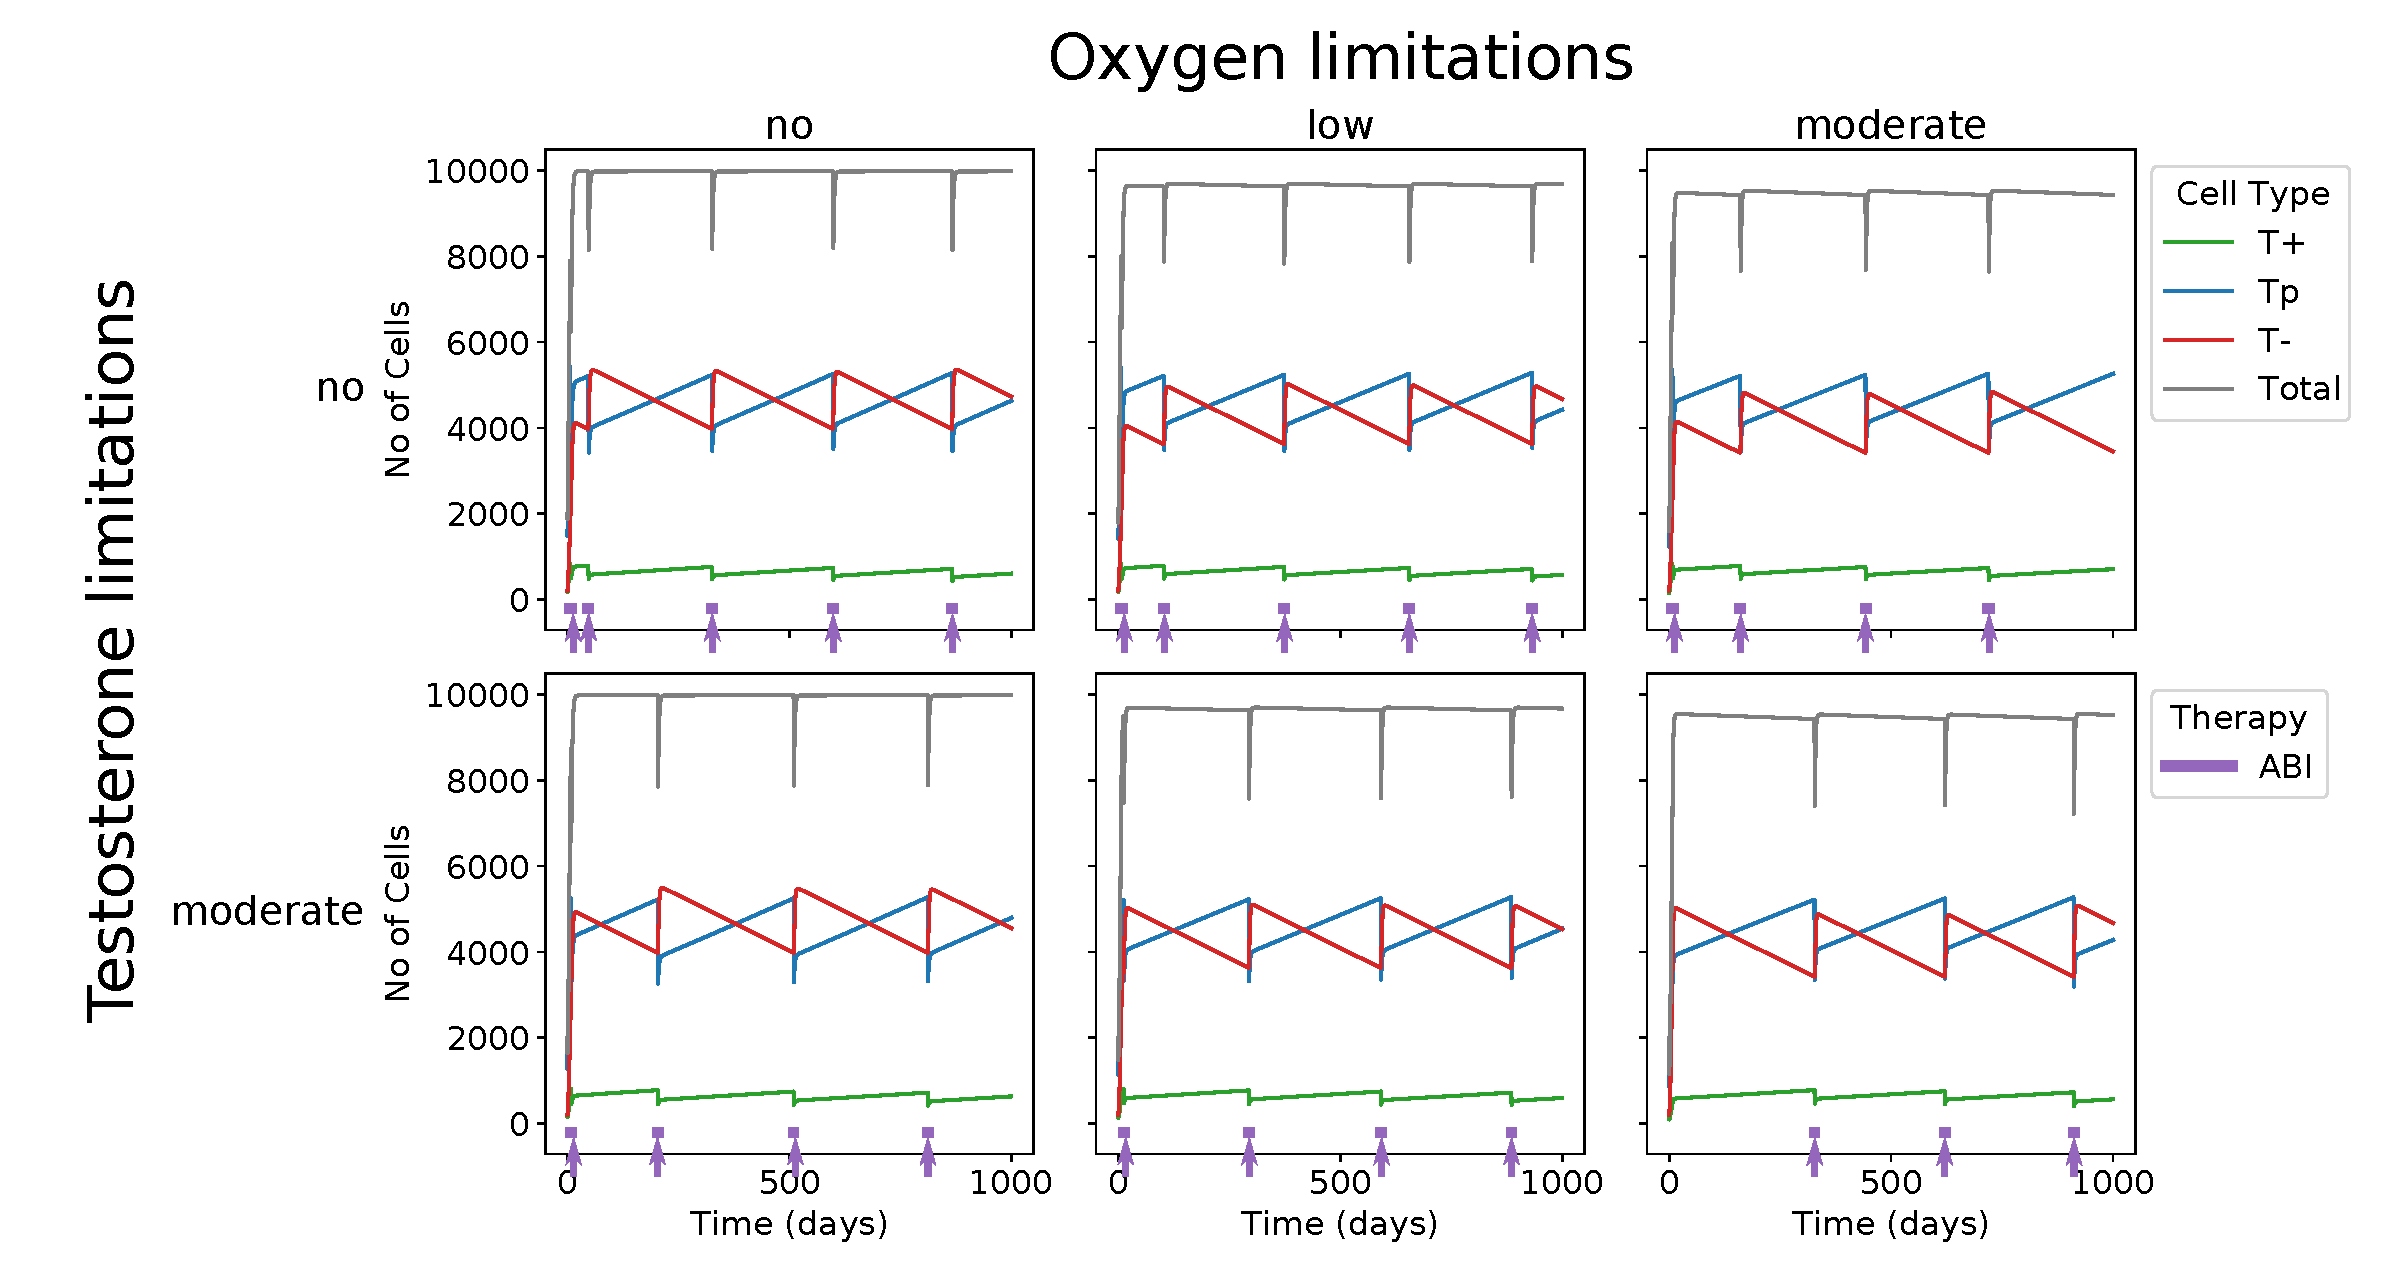
\includegraphics[width=\textwidth]{All3_therapy_8:1:1-2000}
        \caption{High $T^p$ seeding - 8:1:1}
      \end{subfigure}
    \end{adjustwidth}
    \caption{Time-series of all cell types with adaptive therapy. (On:6000, Off:4000)}
  \end{figure}
  \begin{columns}
    \begin{column}{0.5\textwidth}
      \begin{itemize}
        \item<1-> $T^+ - T^p$ extinct just by competition: no effect
        \item<2-> More $T^+ - T^p$ $\rightarrow$ more responsive to abiraterone and better suppress $T^-$
      \end{itemize}
    \end{column}
    \begin{column}{0.5\textwidth}
      \begin{itemize}
        \item<3-> Success of Adaptive therapy:
        \begin{itemize}
          \item<4-> $\checkmark$ Preventing competitive release of resistant
          \item<5-> $\times$ Reducing tumour burden: $T^-$ replace dead cells
        \end{itemize}
      \end{itemize}
    \end{column}
  \end{columns}
\end{frame}

\section{Can adaptive therapy be even made better?}

\begin{frame}{Can delaying treatment help?}
  \begin{figure}[h]
    \begin{adjustwidth}{-5cm}{-5cm}
      \centering
      \begin{subfigure}[b]{0.53\textwidth}
        \centering
        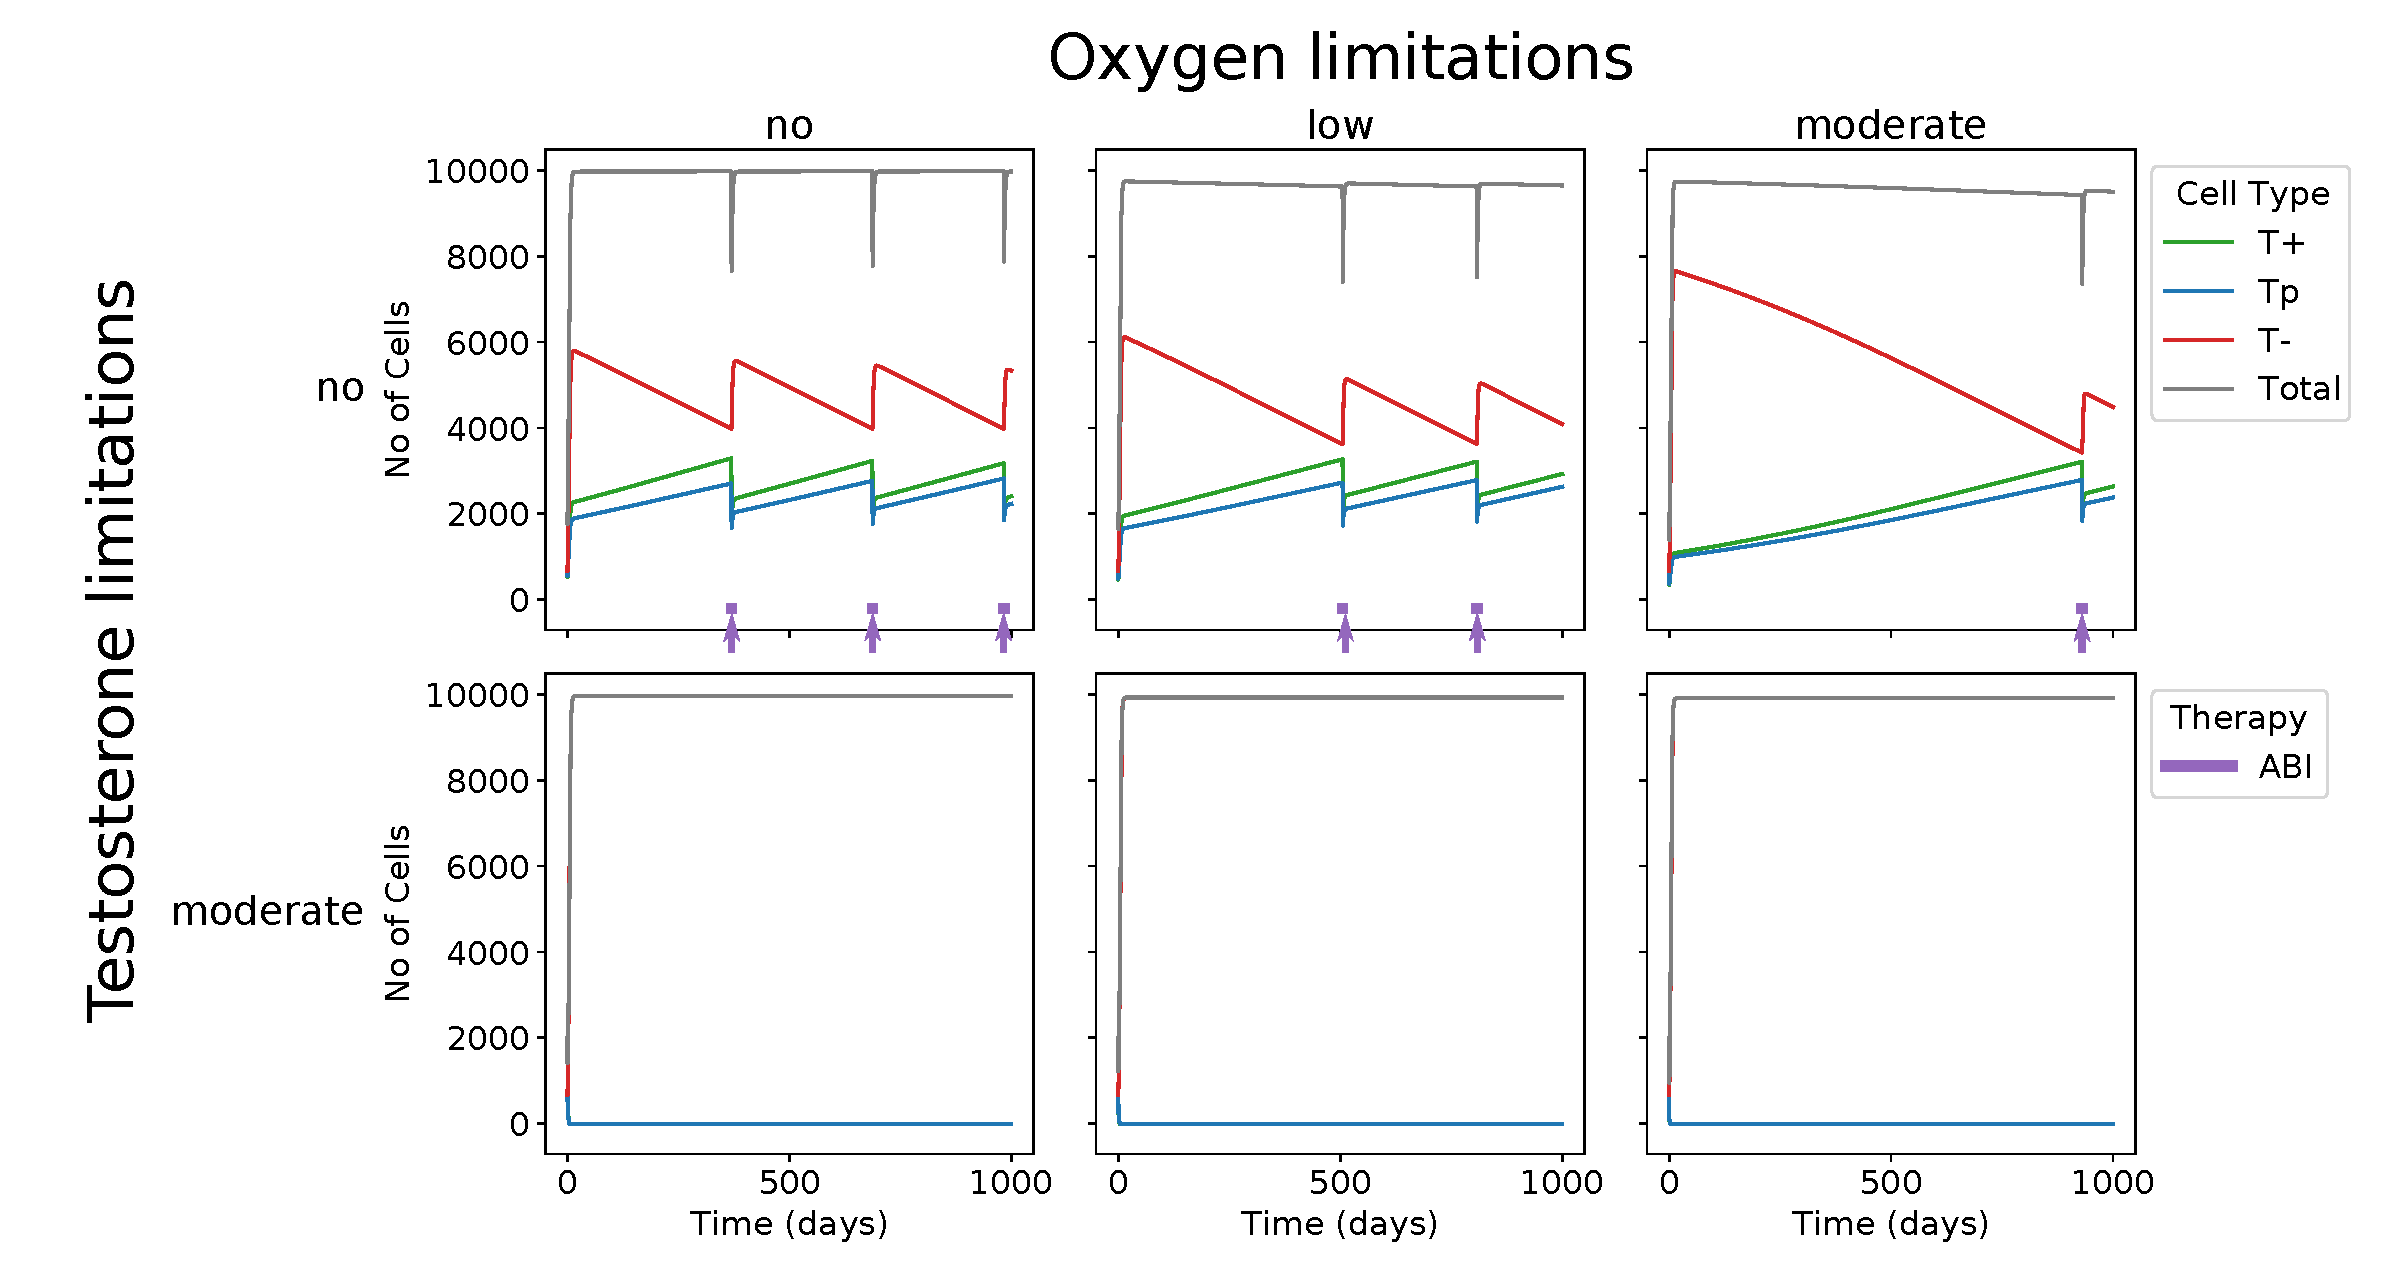
\includegraphics[width=\textwidth]{All3_therapy_200day_1:1:1}
        \caption{Equal seeding - 1:1:1}
      \end{subfigure}
      \begin{subfigure}[b]{0.53\textwidth}
        \centering
        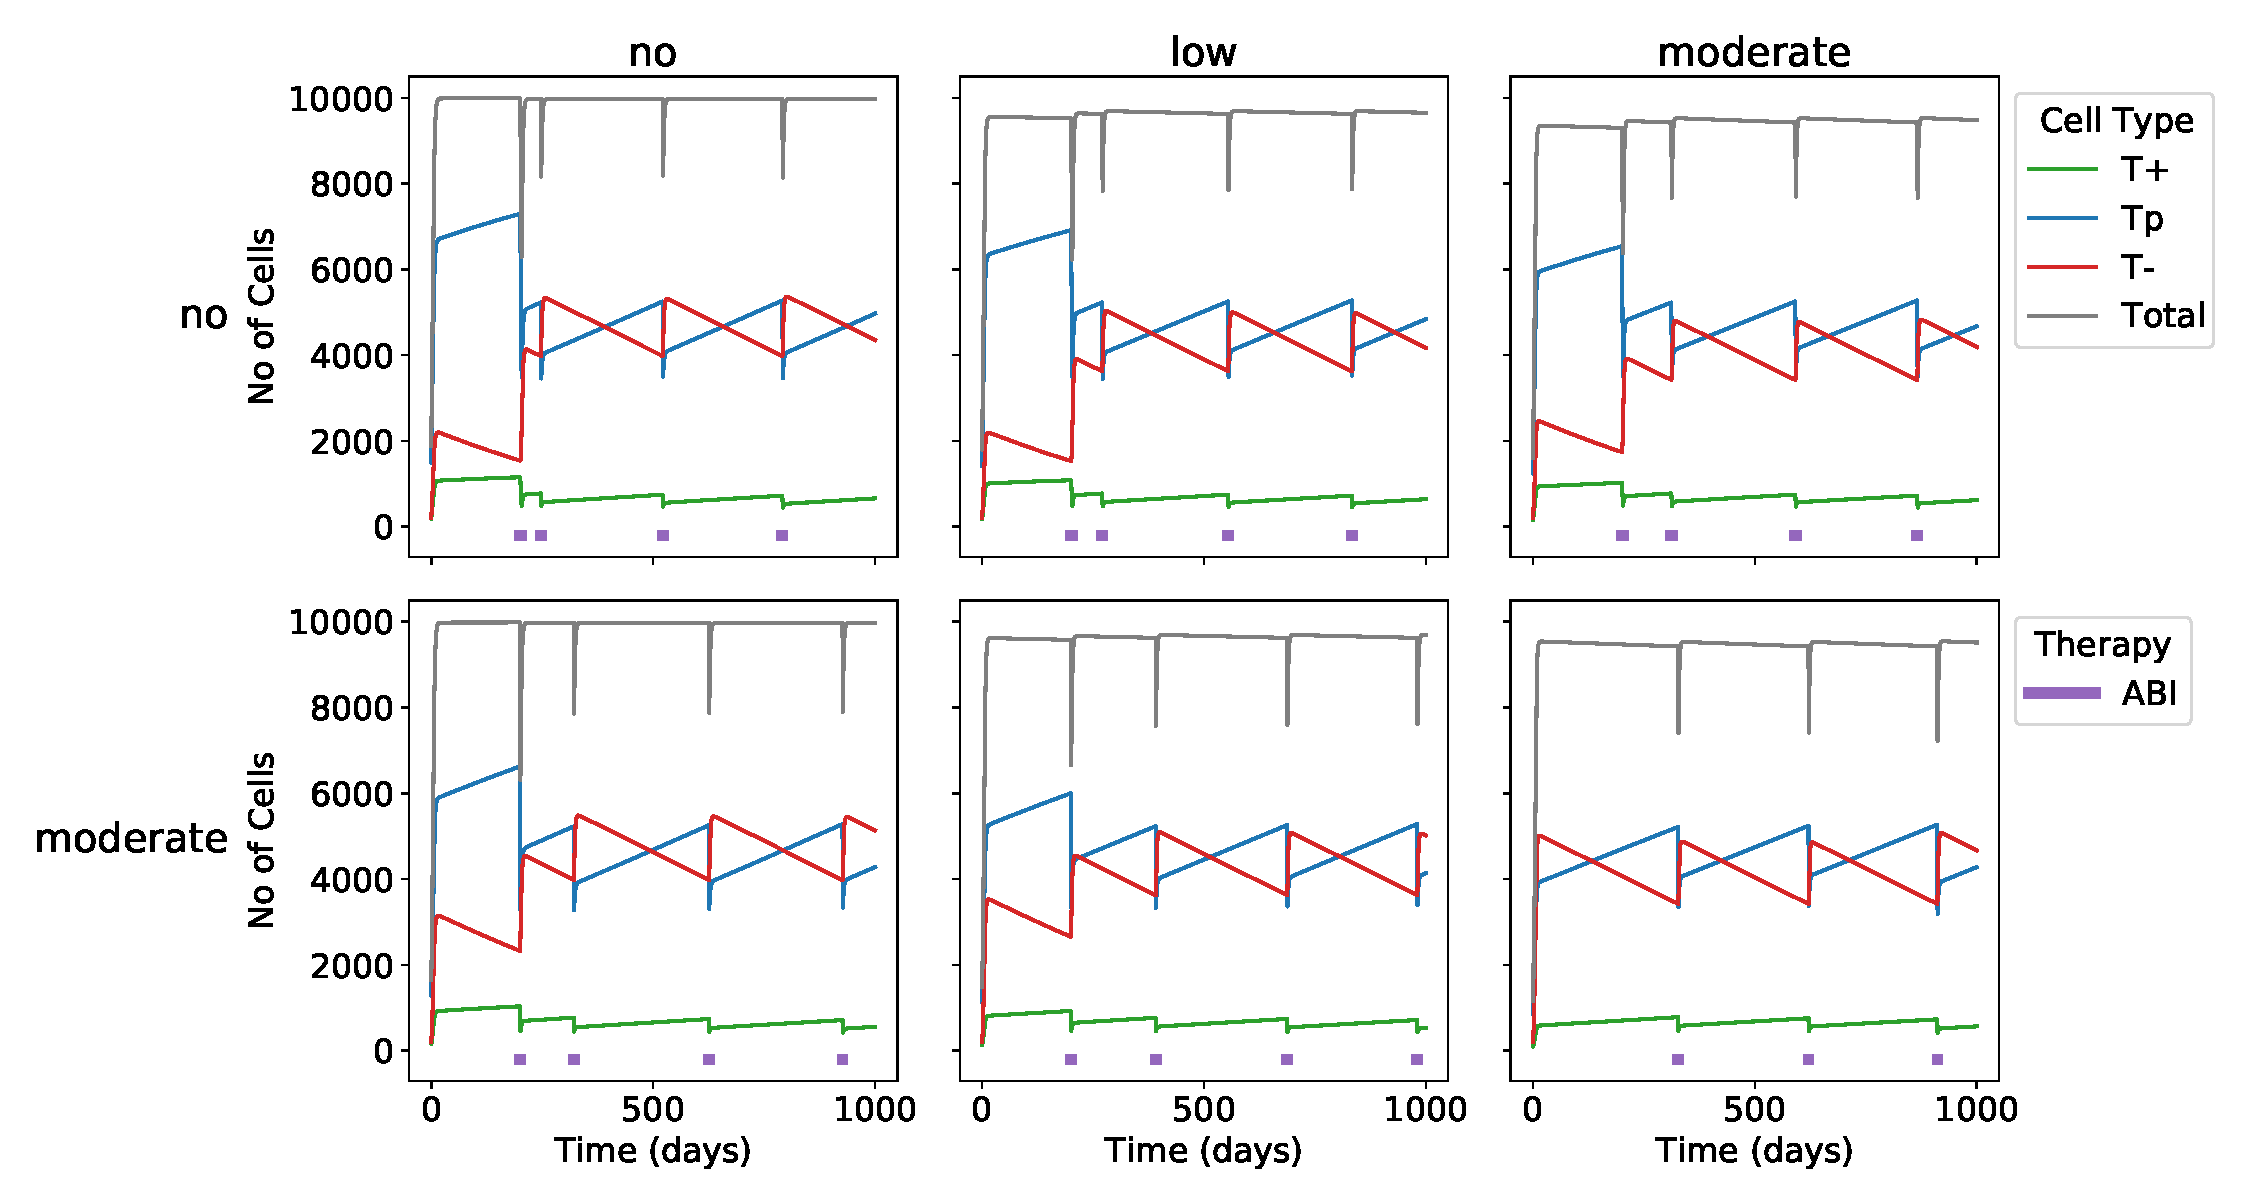
\includegraphics[width=\textwidth]{All3_therapy_200day_8:1:1}
        \caption{High $T^p$ seeding - 8:1:1}
      \end{subfigure}
    \end{adjustwidth}
    \caption{Time-series of all cell types with adaptive therapy delayed by 200 days. (On:6000, Off:4000)}
  \end{figure}
  \begin{columns}
    \begin{column}{0.5\textwidth}
      \begin{itemize}
        \item<1-> $T^+ - T^p$ $\uparrow$ in periods of no therapy
        \item<2-> Speculation: Can delaying bring better balance between $T^+ - T^p$ and $T^-$?
      \end{itemize}
    \end{column}
    \begin{column}{0.5\textwidth}
      \begin{itemize}
        \item<3-> No advantage found as they have similar temporal dynamics
      \end{itemize}
    \end{column}
  \end{columns}
\end{frame}

\begin{frame}{What about using multiple drugs?}
  \begin{figure}[h]
    \begin{adjustwidth}{-5cm}{-5cm}
      \centering
      \begin{subfigure}[b]{0.53\textwidth}
        \centering
        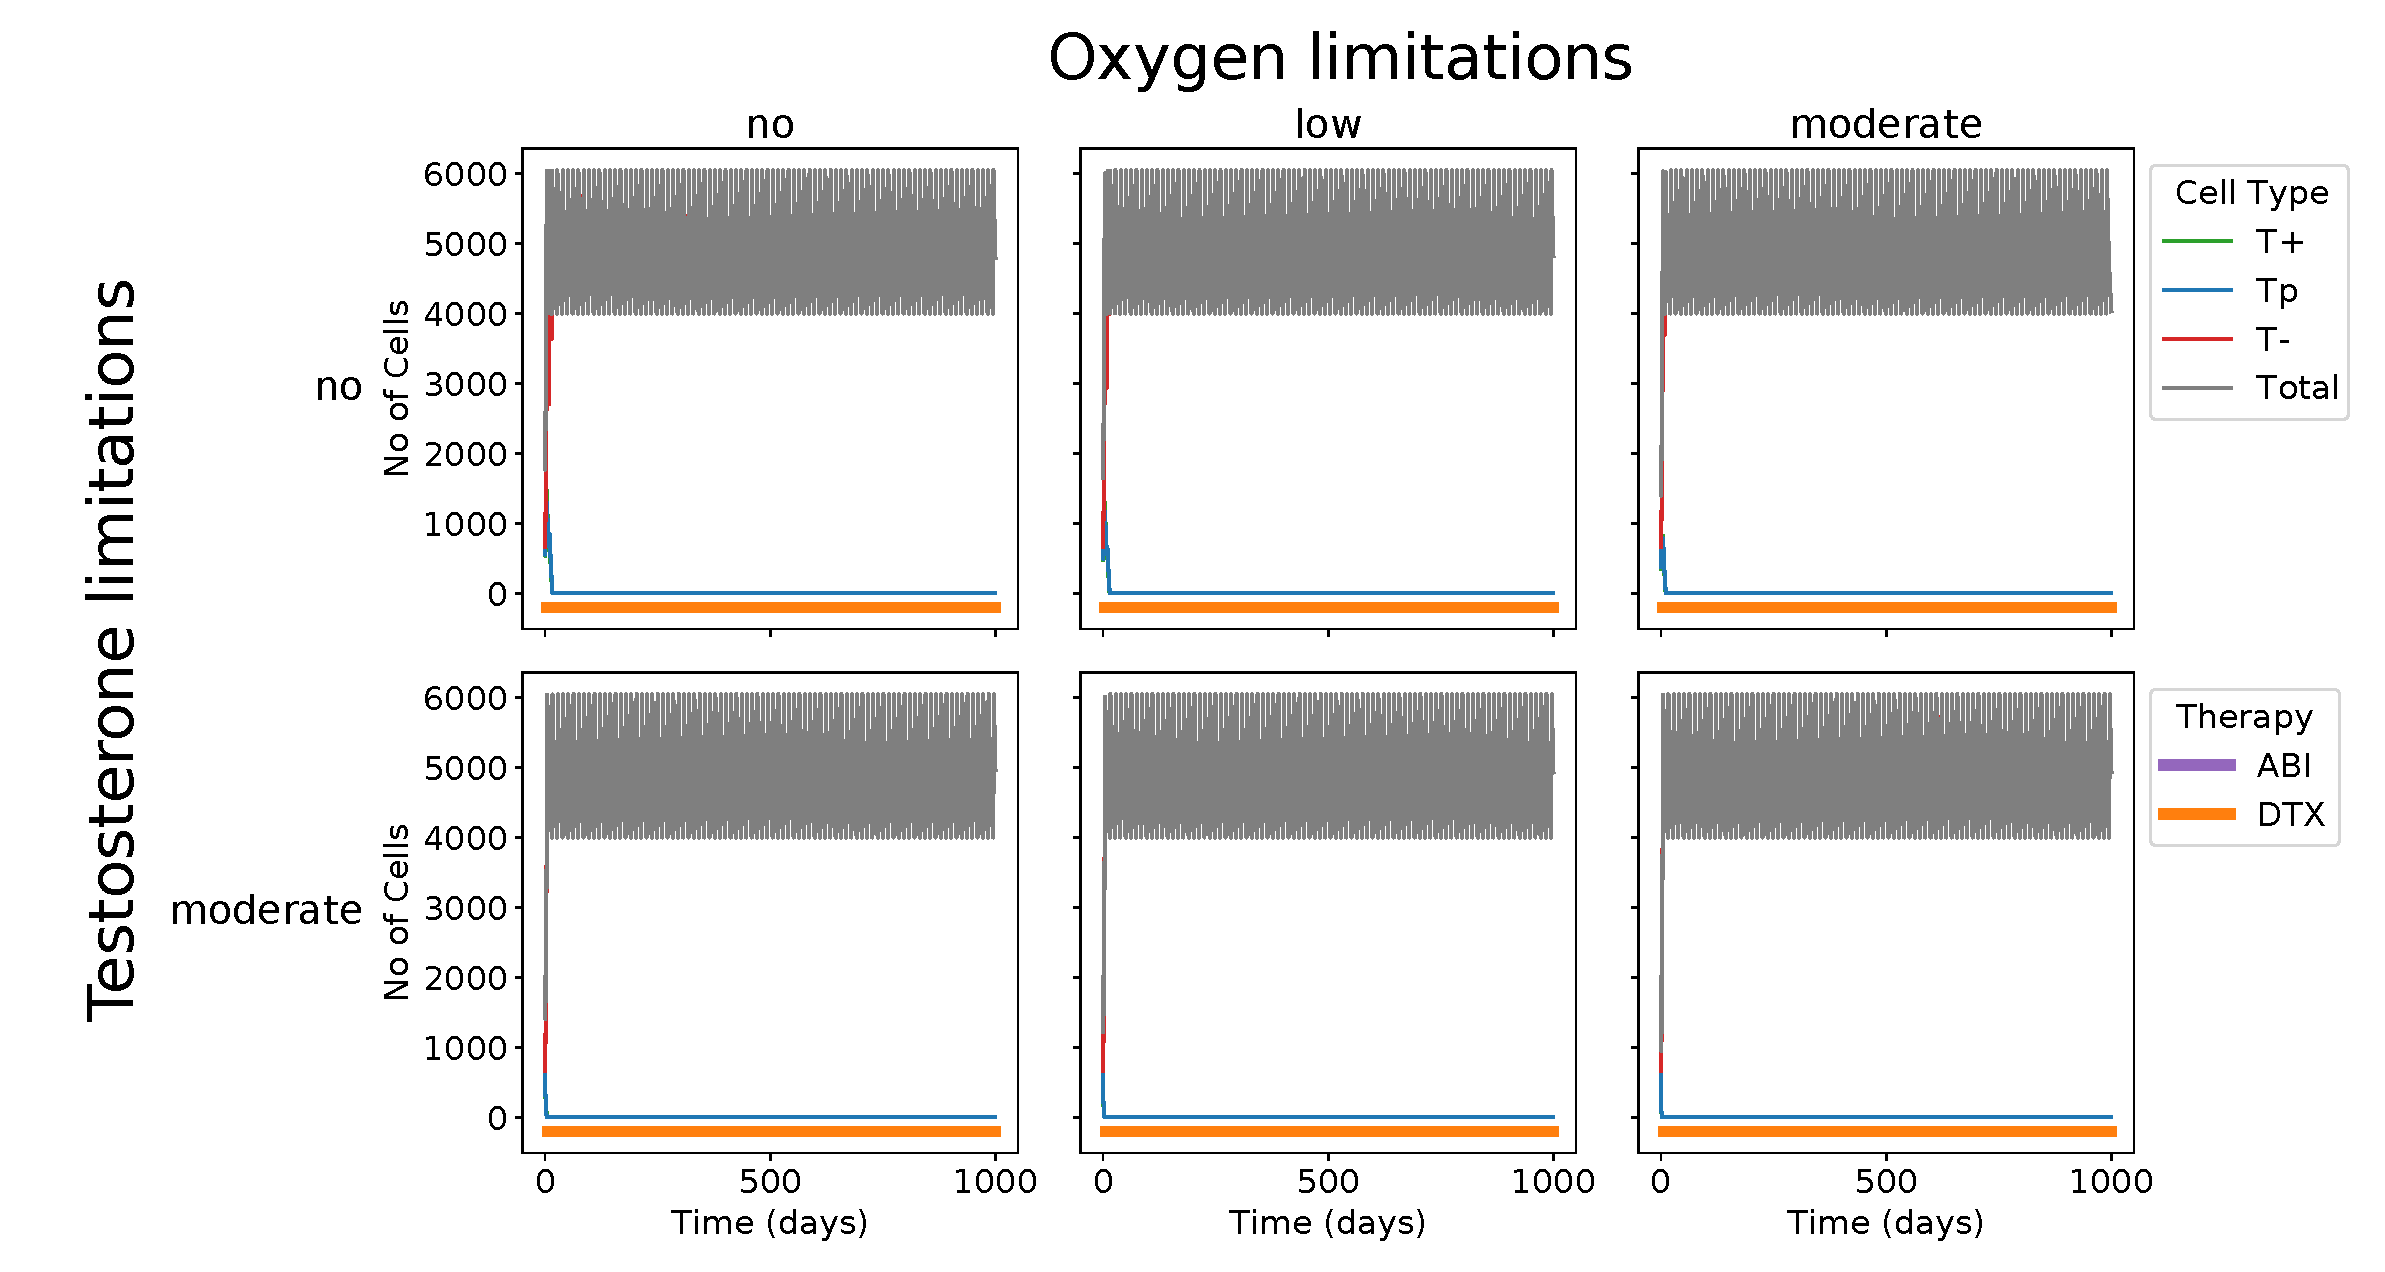
\includegraphics[width=\textwidth]{All3_therapy-combi_1:1:1}
        \caption{Equal seeding - 1:1:1}
      \end{subfigure}
      \begin{subfigure}[b]{0.53\textwidth}
        \centering
        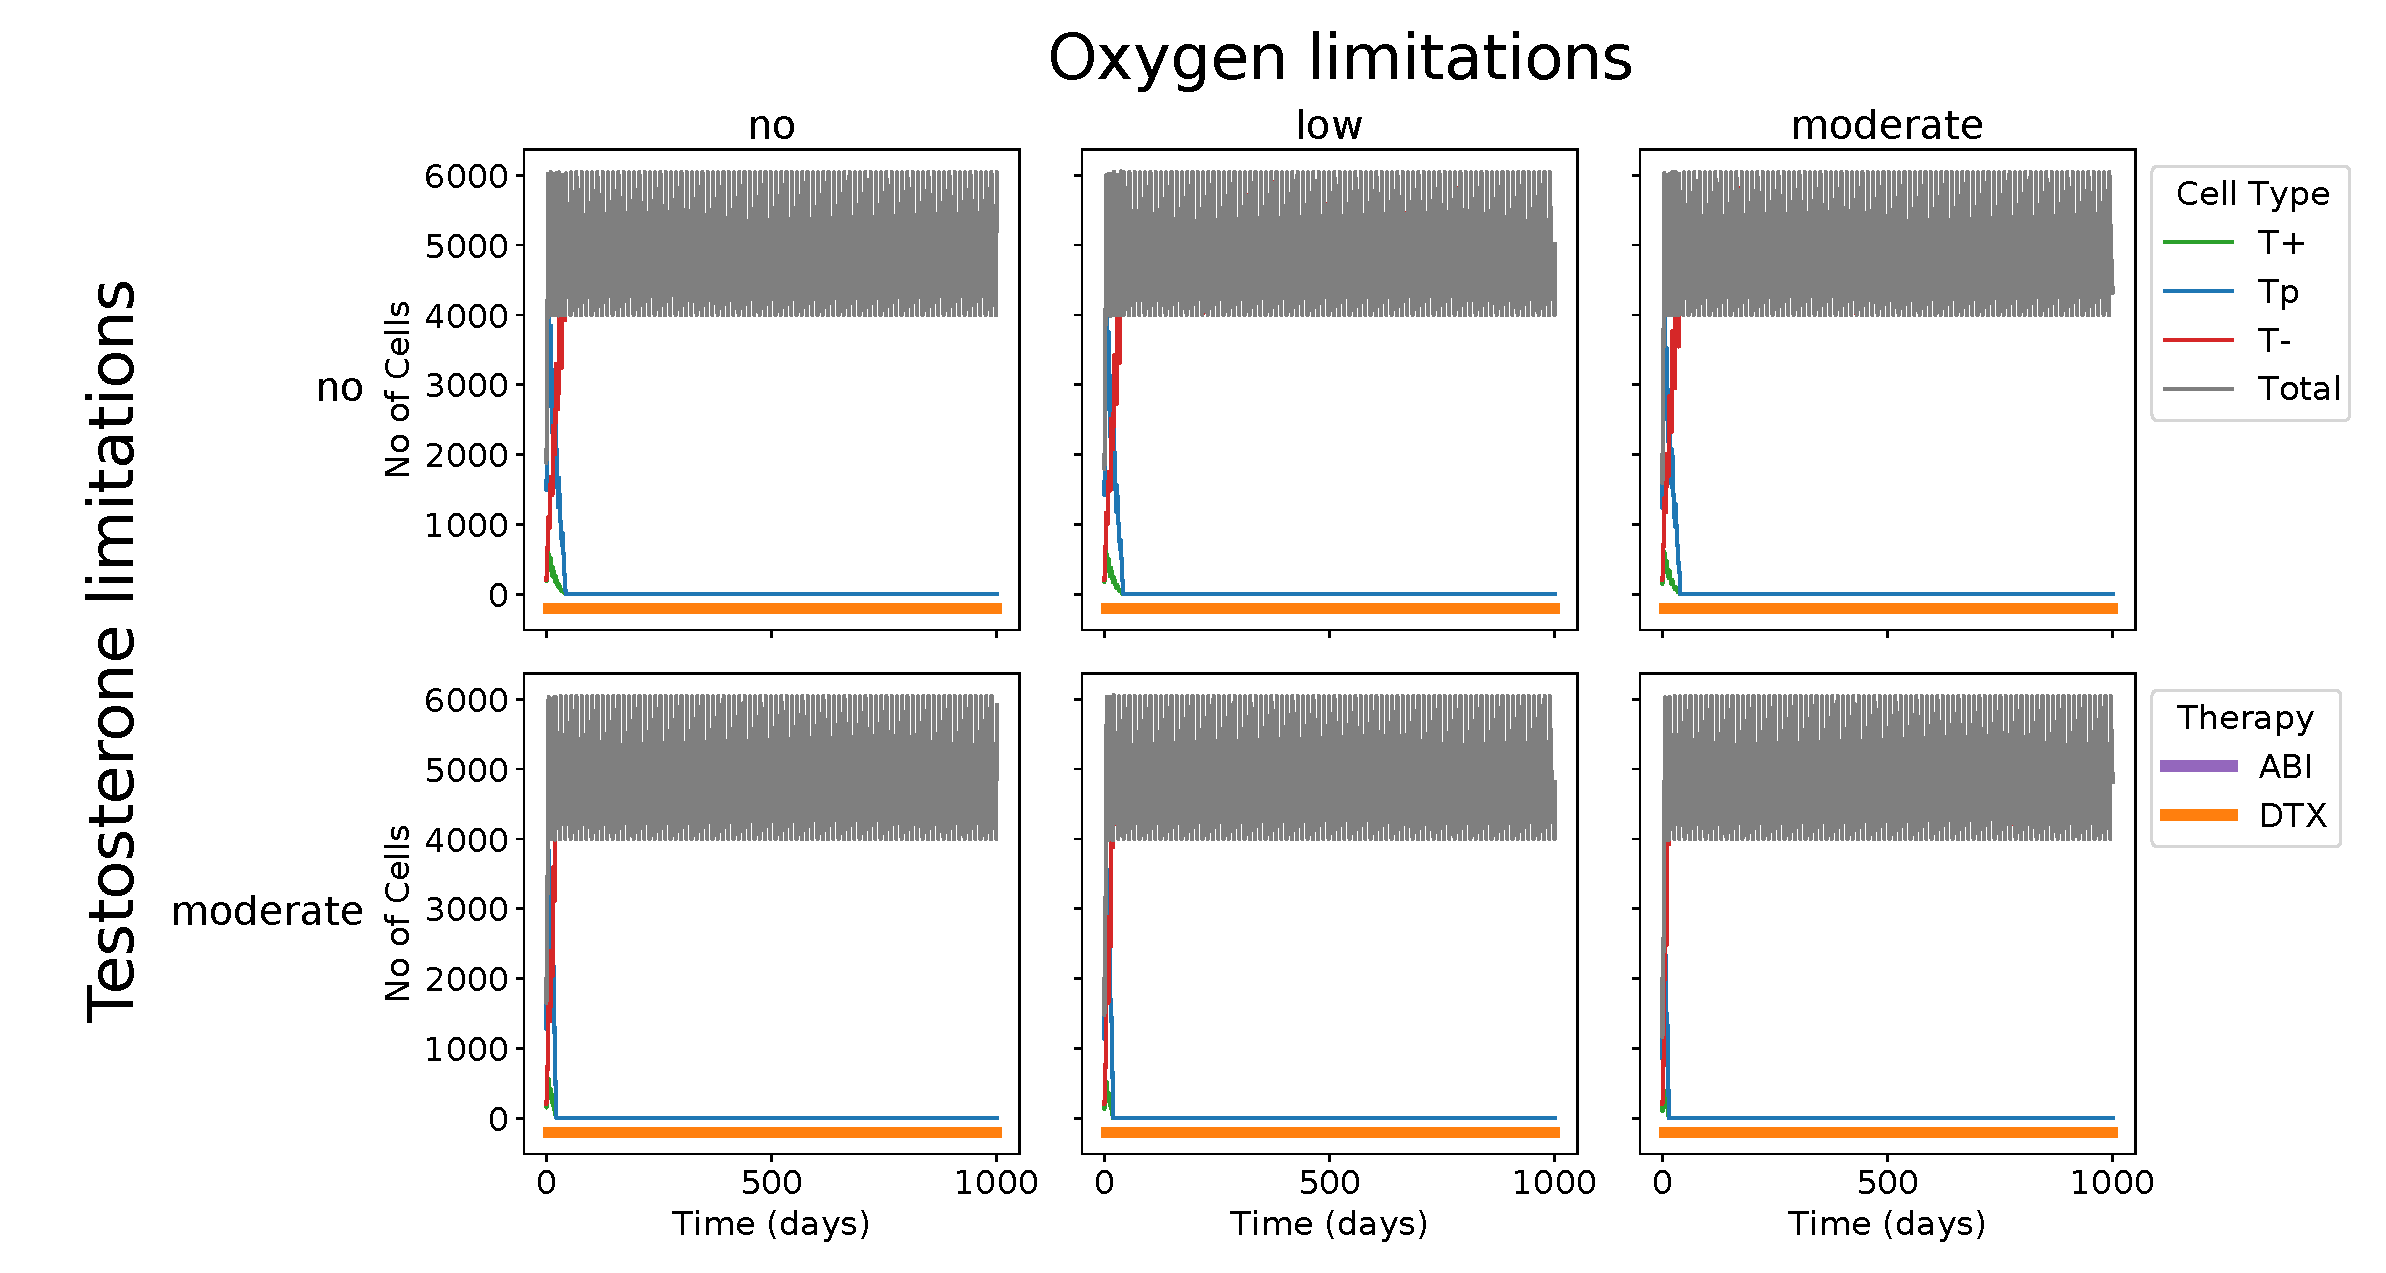
\includegraphics[width=\textwidth]{All3_therapy-combi_8:1:1}
        \caption{High $T^p$ seeding - 8:1:1}
      \end{subfigure}
    \end{adjustwidth}
    \caption{Time-series of all cell types with combination adaptive therapy of abi and dtx\footnotemark[1]. abi(On:6000, Off:4000; $T^+ + T^p$), dtx(On:6000, Off:4000; Total)}
  \end{figure}
  \begin{columns}
    \begin{column}{0.5\textwidth}
      \begin{itemize}
        \item<1-> Hormonal (abi\footnotemark[1]) + cytoxic (dtx\footnotemark[1]) \cite{West}
        \item<2-> Method of action different $\Rightarrow$ Minimal cross resistance
      \end{itemize}
    \end{column}
    \begin{column}{0.5\textwidth}
      \begin{itemize}
        \item<3-> Test-of-concept: would require extensive standardization in future
        \item<4-> $-ve$ effect on coexistence by $\downarrow$ $T^+ - T^p$ outweigh $+ve$ effect on coexistence by $\downarrow$ $T^-$
      \end{itemize}
    \end{column}
  \end{columns}
  \footnotetext[1]{abi: abiraterone, dtx: docetaxel}
\end{frame}


\section{Conclusion}

\begin{frame}{Summary and Future directions}
  \begin{itemize}
    \item<1-> Resource levels can control strength of competition
    \item<2-> Balance of limitations promote coexistence
    \item<3-> With standard-of-care: testosterone limitation is increased leading to extinction
    \item<4-> With adaptive therapy: competitive release avoided
    \begin{itemize}
      \item Effectiveness depends on $T^+$ and $T^p$ population
      \item Population controlled by resource limitations
      \item Maximum limit on $T^+$ and $T^p$ by thresholds of adaptive therapy
    \end{itemize}
    \item<5-> Future directions:
    \begin{itemize}
      \item<6-> Make adaptive therapy effective at reducing tumour burden
      \item<7-> Dynamic thresholds for turning on/off based on composition of the tumour
      \item<8-> Different limitations for different cell types
    \end{itemize}
  \end{itemize}
\end{frame}

\begin{frame}{Acknowledgement}
  I would like to thank the following people:
  \begin{itemize}
    \item Supervisor: Prof. Sutirth Dey
    \item Expert: Dr. M.S. Madhusudhan
    \item Mentor: Vibishan B
    \item PBL Members
    \item Friends and Family
    \item KVPY and IISER Pune
  \end{itemize}
\end{frame}


\begin{frame}[allowframebreaks]
  \printbibliography
\end{frame}

\end{document}
